
\chapter{Applications to Some Nondegenerate problems}\label{chap3}

The\pageoriginale AIM of this Chapter is to show how to apply the general results of
Chapter \ref{chap2}, \ref{chap2-sec4}, to the one-parameter nonlinear
problems introduced in Chapter \ref{chap1}. Such an application is
possible either directly or after a preliminary change of the
parameter. We answer such questions as getting an upper and a
nontrivial lower bound for the {\em number of curves}, their {\em
  regularity} and their {\em location} in space. We have limited
ourselves to the study of two problems, presented in $\S \S 2$ and 3
respectively. These examples are drawn from a global synthetic
approach developed in Rabier \cite{31}, whose technicalities see to be too
tedious to be wholly reproduced here.

In the first section, we prove a generalization of Theorem
\ref{chap1-thm3.2} of Chapter \ref{chap1}. This generalization is of
interest because it shows that when the results of Chapter
\ref{chap2}, $\S 4$, are applied to a mapping $f$ which is the reduced
mapping of some problem posed between real Banach spaces, the
assumptions on $f$ are {\em independent of the Lyapunov-Schmidt
  reduction } used for reducing the problems to a finite-dimensional
one.

The second section is devoted to problems of bifurcation from the {\em
trivial branch} at a {\em multiple characteristic value}. As the Morse
lemma was shown to provide the results of Crandall and Rabinnowitz
when the characteristic value is simple (cf. Chapter \ref{chap1}), the
use of the extended\pageoriginale version yields again, with various
additional improvements, the conclusions of the earlier work by Mc
Leod and Sattinger in their study of the same problem (\cite{23}). Thus,
the analysis of bifurcation from the trivial branch at a simple or
multiple characteristic value appears to follow from the {\em same
  general statement}, giving some homogeneity to the presentation.

In the second section, we consider another example, in which no branch
of solutions is known a priori. In the simplest form of the problem,
two typical situations are those when the origin is a {\em ``turning
  point''} or a {\em ``hystersis point''}. These notions are made
precise and the structure of the local zero set is also determined in
the presence of a higher order singularity. In particular, it is shown
that bifurcation can be expected in this case.

\section{Equivalence of Two Lyapunov-Schmidt Reductions.}\label{chap3-sec1}

Here, we shall define and prove the equivalence of any two
Lyapunov-Schmidt reductions of a given problem. The notion of
equivalence is a key tool for proving a general version of Theorem
\ref{chap1-thm3.2} of Chapter \ref{chap1}. The results of this section
are due to W.J. Beyn \cite{42}.

Let then $\widetilde{X}$ and $Y$ be two real Banach spaces and $G :
\widetilde{X} \to Y$\footnote{Actually, the mapping $G$ needs only to be
defined in a neighbourhood of the origin.} a mapping of class $C^{m}$,
$m \geq 1$, satisfying the conditions:
\begin{equation*}
G(0) = 0,\tag{1.1}\label{chap3-eq1.1}
\end{equation*}

\begin{equation*}
DG(0) \text{ is a Fredholm operator with index 1.}\tag{1.2}\label{chap3-eq1.2}
\end{equation*}\pageoriginale

As in Chapter \ref{chap1}, we shall set
\begin{align*}
\widetilde{X}_{1} & = \text{ Ker } DG(0),\tag{1.3}\label{chap3-eq1.3}\\
Y_{2} & = \text{ Range } DG(0),\tag{1.4}\label{chap3-eq1.4}
\end{align*}
so that $Y_{2}$ has finite codimension $n \geq 0$ and
$\widetilde{X}_{1}$ has finite dimension $n + 1$ from the assumption
(\ref{chap3-eq1.2}). Given two topological complements
$\widetilde{X}_{2}$ and $Y_{1}$ of $\widetilde{X}_{1}$ and $Y_{2}$
respectively, recall that $Q_{1}$ and $Q_{2}$ denote the (continuous)
projection operators onto $Y_{1}$ and $Y_{2}$ respectively and that,
writing $\widetilde{x} \epsilon \widetilde{X}$ in the form
$\widetilde{x} = \widetilde{x}_{1} + \widetilde{x}_{2}$, the reduced
mapping is defined by
\begin{equation*}
\widetilde{x}_{1} \epsilon \widetilde{X}_{1} \to f(x_{1}) =
Q_{1}G(\widetilde{x}_{1} + \widetilde{\varphi}(\widetilde{x}_{1}))
\epsilon Y_{1},\tag{1.5}\label{chap3-eq1.5}
\end{equation*}
where the mapping $\widetilde{\varphi}$ with values in the space
$\widetilde{X}_{2}$ is characterized by 
\begin{equation*}
Q_{2}G(\widetilde{x}_{1} + \widetilde{\varphi}(\widetilde{x}_{1})) = 0,\tag{1.6}\label{chap3-eq1.6}
\end{equation*}
for $\widetilde{x}_{1}$ around the origin in the space
$\widetilde{X}_{1}$ (so that the reduced mapping $f$ in
(\ref{chap3-eq1.5}) is actually defined in a neighbourhood of the
origin in $\widetilde{X}_{1}$). In Theorem \ref{chap3-thm1.1} below,
we show that the mappings $G(\widetilde{x})$ and $f(\widetilde{x}_{1})
+ DG(0) \cdot \widetilde{x}_{2}$ differ only in the context of
``changes of variables'' in the spaces $\widetilde{X}$ and $Y$. More
precisely,

\begin{theorem}\label{chap3-thm1.1}
There is a neighbourhood $\widetilde{U}$ of the origin in the space
$\widetilde{X}$\pageoriginale and
\begin{enumerate}
\item[(i)] a mapping $\tau \epsilon C^{m-1} (\widetilde{U}, Isom
  (Y))$,

\item[(ii)] an origin-preserving diffeomorphism $\widetilde{\rho}
  \epsilon C^{m} (\widetilde{U}, \widetilde{X})$ with
  $D\widetilde{\rho}(0) = I_{\widetilde{X}}$ such that
\begin{equation*}
\widetilde{\tau}(\widetilde{X}) G(\widetilde{\rho}(\widetilde{x})) =
f(\widetilde{x}_{1}) + DG(0) \widetilde{x}_{2},\tag{1.7}\label{chap3-eq1.7}
\end{equation*}
for every $\widetilde{x} \epsilon \widetilde{U}$.
\end{enumerate}
\end{theorem}

\begin{proof}
For $\widetilde{x}$ around the origin in the space $\widetilde{X}$,
set 
\begin{equation*}
\widetilde{R} (\widetilde{x}) = \widetilde{x}_{1} + \left[DG(0)
  |_{\widetilde{X}_{2}}\right]^{-1}
Q_{2}G(\widetilde{x}).\tag{1.8}\label{chap3-eq1.8} 
\end{equation*}

Then, the mapping $\widetilde{R}$ is of class $C^{m}$ and
$\widetilde{R}(0) = 0$, $D\widetilde{R}(0) = I_{\widetilde{X}}$ so
that $\widetilde{R}$ is on origin-preserving local
$C^{m}$-diffeomorphism of the space $\widetilde{X}$. Besides, from
(\ref{chap3-eq1.8}), we have
$$
Q_{2}\widetilde{R}(\widetilde{x}) = \left[DG(0)
  |_{\widetilde{X}_{2}}\right]^{-1} Q_{2}G(\widetilde{x})
$$
and hence
$$
DG(0) Q_{2}\widetilde{R}(\widetilde{x}) = Q_{2}G(\widetilde{x}).
$$

Setting $\widetilde{\rho} = \widetilde{R}^{-1}$, it follows that
\begin{equation*}
Q_{2}G(\widetilde{\rho}(\widetilde{x})) =
DG(0)\widetilde{x}_{2},\tag{1.9}\label{chap3-eq1.9} 
\end{equation*}
for $\widetilde{x}$ in some neighbourhood $\widetilde{U}$ of the
origin in $\widetilde{X}$. Note from (\ref{chap3-eq1.8}) that
$\widetilde{\rho}$ is of the form
\begin{equation*}
\widetilde{\rho}(\widetilde{x}) = \widetilde{x}_{1} + \widetilde{\varphi}(\widetilde{x}),\tag{1.10}\label{chap3-eq1.10}
\end{equation*}
with $\widetilde{\varphi} \epsilon C^{m} (\widetilde{U},
\widetilde{X}_{2})$. In particular, putting $\widetilde{x} =
\widetilde{x}_{1}$ in (\ref{chap3-eq1.9}) (i.e. $\widetilde{x}_{2} =
0$), we find that $\widetilde{\varphi}(\widetilde{x}_{1})$ is
characterized by (\ref{chap3-eq1.6}), which agrees with\pageoriginale
our notation. Besides
\begin{equation*}
\rho(\widetilde{x}_{1}) = Q_{1}G(\widetilde{\rho}(\widetilde{x}_{1})).\tag{1.11}\label{chap3-eq1.11}
\end{equation*}

It is not restrictive to assume that the neighbourhood $\widetilde{U}$
is convex. Let us then define
\begin{equation*}
\tau(\widetilde{x}) = Q_{1} + \tau_{12} (\widetilde{x}) Q_{2} +
Q_{2}\tag{1.12}\label{chap3-eq1.12} 
\end{equation*}
where $\tau_{12}^{(\widetilde{x})} \epsilon \mathscr{L} (Y_{2},
Y_{1})$ is given by
\begin{equation*}
\tau_{12} (\widetilde{x}) = -\left[\int_{0}^{1}
  Q_{1}DG(\widetilde{\rho}(\widetilde{x}_{1} + s\widetilde{x}_{2}))
  D_{\widetilde{x}_{2}} \widetilde{\rho}(\widetilde{x}_{1} +
  s\widetilde{x}_{2}) dx\right] \left[DG(0)
  |_{\widetilde{X}_{2}}\right]^{-1}.\tag{1.13}\label{chap3-eq1.13} 
\end{equation*}

Clearly, $\tau \epsilon C^{m-1} (\widetilde{U}, \mathscr{L}(Y))$ and
$\tau(0) = I_{Y}$ so that, after shrinking $\widetilde{U}$ if
necessary, $\tau(\widetilde{x})$ is an isomorphism of  $Y$ for every
$\widetilde{x} \epsilon \widetilde{U}$. Now, we have
\begin{align*}
\tau(\widetilde{x}) G(\widetilde{\rho}(\widetilde{x})) & =
Q_{1}G(\widetilde{\rho}(\widetilde{x})) + \tau_{12}(\widetilde{x})
Q_{2}G(\widetilde{\rho}(\widetilde{x})) +
Q_{2}G(\widetilde{\rho}(\widetilde{x})) =
\tag{1.14}\label{chap3-eq1.14}\\
& = Q_{1}G(\widetilde{\rho}(\widetilde{x})) + \tau_{12}(\widetilde{x})
DG(0) \widetilde{x}_{2} + DG(0) \widetilde{x}_{2}.
\end{align*}

From (\ref{chap3-eq1.11}) and the Taylor formula, we have
$$
Q_{1}G(\widetilde{\rho}(\widetilde{x})) = f(\widetilde{x}_{1}) +
\int_{0}^{1} Q_{1}DG(\widetilde{\rho}(\widetilde{x}_{1} +
s\widetilde{x}_{2})) D_{\widetilde{x}_{2}}
\widetilde{\rho}(\widetilde{x}_{1} + s\widetilde{x}_{2}) \cdot
\widetilde{x}_{2} dx,
$$
and the assertion follows from (\ref{chap3-eq1.13}) and
(\ref{chap3-eq1.14}).
\end{proof}

By definition, $\widetilde{\rho} = \widetilde{R}^{-1}$ and if we
denote by $\widetilde{R}_{1}$ and $\widetilde{R}_{2}$ the projections
of the mapping $\widetilde{R}$ onto the spaces $\widetilde{X}_{1}$ and
$\widetilde{X}_{2}$ respectively, we can then write for
$\widetilde{x}$ around the origin,
\begin{equation*}
G(\widetilde{x}) = (\tau(\widetilde{x}))^{-1}
\left[f(\widetilde{R}_{1}(\widetilde{x})) + DG(0) \widetilde{R}_{2}\right].\tag{1.15}\label{chap3-eq1.15}
\end{equation*}

Let\pageoriginale us now consider a second Lyapunov-Schmidt reductions
corresponding to a new choice $\widetilde{X}'_{2}$ of the complement
of $\widetilde{X}_{1}$ and a write $\widetilde{x} = \widetilde{x}'_{1}
+ \widetilde{x}'_{2}$ with $\widetilde{x}'_{1} \epsilon
\widetilde{X}_{1}$ and $\widetilde{x}'_{2} \epsilon
\widetilde{X}'_{2}$. We obtain a new reduced equation $\hat{f} =
\hat{f}(\widetilde{x}'_{1})$ with which Theorem \ref{chap3-thm1.1}
applies. Together with (\ref{chap3-eq1.15}), we see that there is a
neighbourhood $\widetilde{U}$ of the origin in the space
$\widetilde{X}$ and 
\begin{enumerate}
\item[(i)] a mapping $\tau \epsilon C^{m-1}(\widetilde{U}, Isom (Y))$,

\item[(ii)] an origin-preserving diffeomorphism $\widetilde{\rho}
  \epsilon C^{m} (\widetilde{U}, \widetilde{X})$ with onto the spaces
  $\widetilde{X}_{1}$ and $\widetilde{X}_{2}$ respectively, one has
\begin{equation*}
\hat{f}(\widetilde{x}'_{1}) + DG(0)\widetilde{x}'_{2} =
\tau(\widetilde{x}) \left[f(\widetilde{\rho}_{1}(\widetilde{x})) + DG(0)\widetilde{\rho}(\widetilde{x})\right],\tag{1.16}\label{chap3-eq1.16}
\end{equation*}
for every $\widetilde{x} \epsilon \widetilde{U}$. The linear mapping
$\tau(\widetilde{x})$ has a matrix representation of the form
\begin{equation*}
\tau(\widetilde{x}) = 
\begin{bmatrix}
\hat{\tau}_{11}(\widetilde{x}) & \hat{\tau}_{12}(\widetilde{x})\\
\tau_{21}(\widetilde{x}) & \tau_{22}(\widetilde{x})\\
\end{bmatrix}
,
\end{equation*}
where $\hat{\tau}_{1i} \epsilon C^{m-1}(\widetilde{U}, (Y_{i},
\hat{Y}_{1})), i = 1, 2$ and $\tau_{2i} \epsilon
C^{m-1}(\widetilde{U}, (Y_{i}, Y_{2})), i = 1, 2$. In this notation,
relation (\ref{chap3-eq1.16}) can be rewritten as
\begin{align*}
& \hat{f}(\widetilde{x}'_{1}) = \hat{\tau}_{11}(\widetilde{x})
  f(\widetilde{\rho}_{1}(\widetilde{x})) +
  \hat{\tau}_{12}(\widetilde{x}) DG(0)
  \widetilde{\rho}_{2}(\widetilde{x}),\tag{1.17}\label{chap3-eq1.17}\\
& DG(0) \widetilde{x}'_{2} = \tau_{21}(\widetilde{x})
  f(\widetilde{\rho}_{1}(\widetilde{x})) + \tau_{22}(\widetilde{x})
  DG(0) \widetilde{\rho}_{2} (\widetilde{x}),\tag{1.18}\label{chap3-eq1.18}
\end{align*}
for every $\widetilde{x} \epsilon \widetilde{U}$.
\end{enumerate}

Assume\pageoriginale first that $m \geq 2$, so that the mappings
$\tau_{21}$ and $\tau_{22}$ are of class $C^{1}$ at least. By
differentiating (\ref{chap3-eq1.18}) and noting that
$D\widetilde{\rho}(0) = I_{\widetilde{x}}$, we obtain
\begin{equation*}
DG(0) \widetilde{P}'_{2} = \tau_{21}(0) Df(0) + \tau_{22}(0) DG(0)
\widetilde{P}_{2},\tag{1.19}\label{chap3-eq1.19} 
\end{equation*}
where $\widetilde{P}_{2}$ and $\widetilde{P}'_{2}$ denote the
projection operators along $\widetilde{X}_{1}$ and onto the spaces
$\widetilde{X}_{2}$ and $\widetilde{X}'_{2}$ respectively. When $m =
1$, the mappings $\tau_{21}$ and $\tau_{22}$ are of class $C^{0}$
only. Nevertheless, from the fact that the mappings $f \cdot
\widetilde{\rho}_{1}$ and $DG(0) \cdot \widetilde{\rho}_{2}$ are of
class $C^{1}$ and {\em vanish at the origin}, it is immediately
verified that both the mapping
$$
\widetilde{x}_{2} \to \tau_{21}(\widetilde{x}_{2})
f(\widetilde{\rho}_{1} (\widetilde{x})),
$$
and
$$
\widetilde{x}_{2} \to \tau_{22}(\widetilde{x}) DG(0) \widetilde{\rho}_{2}(\widetilde{x}),
$$
are differntiable at the origin and that formula (\ref{chap3-eq1.19})
still holds. Besides, $Df(0) = 0$ (cf, Chapter \ref{chap1}, $\S 2$)
and hence
$$
DG(0) \widetilde{P}'_{2} = \tau_{22}(0) DG(0) \widetilde{P}_{2}.
$$

In particular,
$$
DG(0) \widetilde{P}'_{2} |_{\widetilde{X}_{2}} = \tau_{22}(0) DG(0)
|_{\widetilde{X}_{2}}. 
$$

As $DG(0)|_{\widetilde{X}_{2}} \epsilon Isom (\widetilde{X}_{2},
Y_{2})$, we get
\begin{equation*}
\tau_{22}(0) = \left[DG(0) |_{\widetilde{X}_{2}}\right]^{-1} DG(0)
\widetilde{P}'_{2} |_{\widetilde{X}_{2}}.\tag{1.20}\label{chap3-eq1.20}
\end{equation*}

At\pageoriginale this stage, observe that $DG(0) \widetilde{P}'_{2} =
DG(0) |_{\widetilde{X}'_{2}}$. Indeed, as $\widetilde{X}_{2}$ and
$\widetilde{X}'_{2}$ are two topological complements \footnote{In
  particular, $\widetilde{X}_{2}$ and $\widetilde{X}'_{2}$ are closed
  in $\widetilde{X}$ and hence are Banach spaces by themselves.} of
the space $\widetilde{X}_{1}$, it suffices to notice that
$\widetilde{P}'_{2} |_{\widetilde{X}_{2}}$ is onr-to-one and onto and
use the Open mapping theorem. Therefore, writing (\ref{chap3-eq1.20})
in the form
$$
\tau_{22}(0) = \left[DG(0) |_{\widetilde{X}_{2}}\right]^{-1}
\left[DG(0) |_{\widetilde{X}_{2}}\right] P'_{2} |_{\widetilde{X}_{2}},
$$
it follows that $\tau_{22}(0) \epsilon$ Isom  $(Y_{2})$. After
shrinking the neighbourhood $\widetilde{U}$ if necessary, we may then
suppose that $\tau_{22}(\widetilde{x}) \epsilon$ Isom $(Y_{2})$ for
every $\widetilde{x} \epsilon \widetilde{U}$.

Now, let us take $\widetilde{x} \epsilon \widetilde{X}_{1}$
(i.e. $\widetilde{x} = \widetilde{x}_{1} = \widetilde{x}'_{1}$) in
(\ref{chap3-eq1.17}) and (\ref{chap3-eq1.18}) to obtain
\begin{align*}
\hat{f}(\widetilde{x}_{1}) & = \hat{\tau}_{11}(\widetilde{x}_{1})
f(\widetilde{\rho}_{2}(\widetilde{x}_{1})) +
\hat{\tau}_{12}(\widetilde{x}_{1}) DG(0)
\widetilde{\rho}_{2}(\widetilde{x}_{1}),\tag{1.21}\label{chap3-eq1.21}\\
 0  & = \tau_{11}(\widetilde{x}_{1})
f(\widetilde{\rho}_{1}(\widetilde{x}_{1})) +
\tau_{22}(\widetilde{x}_{1}) DG(0)
\widetilde{\rho}_{2}(\widetilde{x}_{1}),\tag{1.22}\label{chap3-eq1.22}
\end{align*}

From (\ref{chap3-eq1.22}) and the above comments, we see that
$$
DG(0) \widetilde{\rho}_{2}(\widetilde{x}_{1}) =
-(\tau_{22}(\widetilde{x}_{1}))^{-1} \tau_{21}(\widetilde{x}_{1}) f(\widetilde{\rho}_{1}(\widetilde{x}_{1})).
$$

With this relation, (\ref{chap3-eq1.21}) becomes
$$
\hat{f}(\widetilde{x}_{1}) = \left[\hat{\tau}_{11} (\widetilde{x}_{1})
- \hat{\tau}_{12}
(\widetilde{x}_{1})(\tau_{22}(\widetilde{x}_{1}))^{-1}
\tau_{21}(\widetilde{x}_{1})\right] f(\widetilde{\rho}_{1}(\widetilde{x}_{1})).
$$

Let us set
$$
\hat{\tau}(\widetilde{x}_{1}) = \hat{\tau_{11}}(\widetilde{x}_{1}) -
\hat{\tau}_{12}(\widetilde{x}_{1})(\tau_{22}(\widetilde{x}_{1}))^{-1} \tau_{21}(\widetilde{x}_{1}).
$$

Clearly,\pageoriginale $\hat{\tau}_{1}$ is of class $C^{m-1}$ on a
neighbourhood of the origin in the space $\widetilde{X}_{1}$ with
values in the space $\mathscr{L}(Y_{1}, \hat{Y}_{1})$. In addition,
$\hat{\tau}_{1}(0) \epsilon$ isom $(Y_{1}, \hat{Y_{1}})$. Indeed,
since $Y_{1}$ and $\hat{Y}_{1}$ have the same dimension $n$, it suffices
to show that $\hat{\tau}_{1} (0)$ is one-to-one. Let $Y_{1} \epsilon
Y_{1}$ be such that $\hat{\tau}_{1} (0)y_{1} = 0$, namely
$$
\hat{\tau}_{11}(0)y_{1} - \hat{\tau}_{12}(0)(\tau_{22}(0))^{-1}
\tau_{21}(0)y_{1} = 0
$$

If so, we seet that
\begin{equation*}
\begin{bmatrix}
\hat{\tau}_{11}(0) & \hat{\tau}_{12}(0)\\
\tau_{21}(0) & \tau_{22}(0)\\
\end{bmatrix}
\begin{bmatrix}
y_{1} & \\
- \left(\tau_{22}(0) \right)^{-1} & \tau_{21}(0)y_{1}
\end{bmatrix}
= 0
\end{equation*}
and hence $y_{1} = 0$. It follows that $\hat{\tau}_{1}(\widetilde{x})
\epsilon$ Isom $(Y_{1}, \hat{Y}_{1})$ for $\widetilde{x}_{1}$ near the
origin in the space $\widetilde{X}_{1}$ and we have proved

\begin{theorem}\label{chap3-thm1.2}
There is a neighbourhood $\widetilde{U}_{1}$ of the origin in the
space $\widetilde{X}_{1}$ and
\begin{enumerate}
\item[(i)] a mapping $\hat{\tau}_{1} \epsilon C^{m-1}
  (\widetilde{U}_{1}, Isom (Y_{1}, \hat{Y}_{1}))$,

\item[(ii)] an origin-preserving diffeomorphism $\widetilde{\rho}_{1}
  \epsilon C^{m} (\widetilde{U}_{1}, \widetilde{X}_{1})$ with\break
  $D\widetilde{\rho}_{1}(0) = I_{\widetilde{X}'_{1}}$ such that
\begin{equation*}
\hat{f}(\widetilde{x}_{1}) = \hat{\tau}_{1}(\widetilde{x}_{1})
f(\widetilde{\rho}_{1} (\widetilde{x}_{1})),\tag{1.23}\label{chap3-eq1.23}
\end{equation*}
\end{enumerate}
for every $\widetilde{x}_{1} \epsilon \widetilde{U}_{1}$.
\end{theorem}

\begin{remark}\label{chap3-rem1.1}
It is customary to summarize Theorem \ref{chap3-thm1.2} by saying that
any two Lyapunov-Schmidt reductions are {\em equivalent}. For our
purpose, this property is important because of Corollary
1.1 below. 
\end{remark}


\setcounter{corollary}{1}
\begin{corollary}\label{chap3-coro1.2}
Assume\pageoriginale that there is an integer $k \leq m$ such that
$$
D^{j}f(0) = 0, 0 \leq j \leq k-1,
$$
and the mapping
\begin{equation*}
\widetilde{x}_{1} \epsilon \widetilde{X}_{1} \to D^{k}f(0) \cdot
(\widetilde{x}_{1})^{k} \epsilon Y_{1},\tag{1.24}\label{chap3-eq1.24}
\end{equation*}
verifies the condition $(\mathbb{R}-N.D.)$. Then, one has
$$
D^{j}\hat{f}(0) = 0, 0 \leq j \leq k-1,
$$
and the mapping
\begin{equation*}
x_{1} \epsilon X_{1} \to D^{k}\hat{f}(0) \cdot (\widetilde{x}_{1})^{k}
\epsilon \hat{Y}_{1},\tag{1.25}\label{chap3-eq1.25}
\end{equation*}
verifies the condition $(\mathbb{R}-N.D.)$.
\end{corollary}

\begin{proof}
With the notation of Theorem \ref{chap3-thm1.2}, note that in view of
$D\widetilde{\rho}_{1} (0) = I_{\widetilde{X}_{1}}$ that
\begin{equation*}
D^{j}(f \bullet \widetilde{\rho}_{1})(0) = D^{j}f(0), 0 \leq j \leq k.\tag{1.26}\label{chap3-eq1.26}
\end{equation*}

Assume first $k \leq m-1$, so that, for every $0 \leq j \leq k$,
$D^{j}\hat{f}(0)$ involves the derivatives of order $\leq k$ of the
mappings $\hat{\tau}_{1}$ and $f \bullet \rho_{1}$ at the origin as it
follows from (\ref{chap3-eq1.23}). With (\ref{chap3-eq1.26}), a simple
calculation provides
\begin{align*}
D^{j}\hat{f}(0) & = 0, 0 \leq j \leq
k-1,\tag{1.27}\label{chap3-eq1.27}\\
D^{k}\hat{f}(0) & = \hat{\tau}_{1}(0) \; D^{k}f(0).\tag{1.28}\label{chap3-eq1.28}
\end{align*}

If $k = m$, there is a slight difficulty in applying the same method
since the mapping $\hat{\tau}_{1}$ is not $m$ times
differentiable. However, it is easy to obtain $D^{m-1}
\hat{f}(\widetilde{x}_{1})$ in terms of the derivatives of order $\leq
m - 1$ of\pageoriginale the mappings $\hat{\tau}_{1}$ and $(f \bullet
\widetilde{\rho}_{1})$. We leave it to the reader to check that each
term of the expression is differentiable {\em at the origin} and the
relations (\ref{chap3-eq1.27}) and (\ref{chap3-eq1.28}) still hold. In
particular, as $\hat{\tau}_{1}(0) \epsilon Isom (Y_{1}, \hat{Y}_{1})$,
it is an obvious consequence of (\ref{chap3-eq1.27}) that the mapping
(\ref{chap3-eq1.25}) verifies the condition $(\mathbb{R}-N.D.)$ as
soon as the mapping (\ref{chap3-eq1.24}) does.
\end{proof}

\begin{remark}\label{chap3-rem1.2}
From Corollary \ref{chap3-coro1.2}, assuming that the first nonzero
derivative at the origin of the reduced mapping $f$ verifies the
condition $(\mathbb{R}-N.D.)$ is independent of the choice of the
spaces $\widetilde{X}_{2}$ and $Y_{1}$ and hence is an {\em intrinsic
  property of the mapping $G$}.
\end{remark}

\section[Application to Problems of Bifurction.....]{Application to Problems of Bifurction from the Trivial Branch
  at a Multiple Characteristic\hfil\break Value}\label{chap3-sec2}

According to our definitions of Chapter \ref{chap1}, given a real
Banach space $X$, we are interested in finding the solutions $(\mu, x)$
near the origin of $\mathbb{R} \times X$ of an equation of the form
\begin{equation*}
G(\mu, x) = (I - (\lambda_{0} + \mu)L) x + \Gamma (\mu, x) = 0,
\tag{2.1}\label{chap3-eq2.1} 
\end{equation*}
where $L \epsilon \mathscr{L}(X)$ is {\em compact} and $\lambda_{0}$
is a {\em multiple} characteristic value of $L$, i.e.,
$$
n = dim Ker (I - \lambda_{0} L) \geq 2.
$$

Recall the notation (cf. Chapter \ref{chap1}):
\begin{align*}
X_{1} & = Ker (I - \lambda_{0}L),\tag{2.2}\label{chap3-eq2.2}\\
Y_{2} & = Range (I - \lambda_{0}L),\tag{2.3}\label{chap3-eq2.3}
\end{align*}
and\pageoriginale $X_{2}$ and $Y_{1}$ are arbitrary topological
complements of $X_{1}$ and $Y_{2}$ respectively. If so,
\begin{equation*}
dim X_{1} = dim Y_{1} = n.\tag{2.4}\label{chap3-eq2.4}
\end{equation*}

Also, $Q_{1}$ and $Q_{2}$ denote the (continuous) projection operators
onto the spaces $Y_{1}$ and $Y_{2}$. The nonlinear operator $\Gamma$
verifies conditions
\begin{equation*}
\Gamma(\mu, 0) = 0,\tag{2.5}\label{chap3-eq2.5}
\end{equation*}
(so that $D_{\mu}^{j} \Gamma(0) = 0$ for every $j \geq 0$) and
\begin{equation*}
D_{x}\Gamma(0) = D_{\mu}D_{x}\Gamma(0) = 0.\tag{2.6}\label{chap3-eq2.6}
\end{equation*}

In what follows, we shall assume that there is an integer $k \leq m$
(and necessarily $\geq 2$) such that
\begin{align*}
& Q_{1}D_{x}^{j}\Gamma(0) = 0, 0 \leq j \leq k-1,\\
& Q_{1}D_{x}^{k}\Gamma(0) |_{(X_{1})^{k}} \neq 0,\tag{2.7}\label{chap3-eq2.7}
\end{align*}

As we saw in Chapter \ref{chap1}, $\S 2$, the problem amounts to
finding the local zero set of the {\em reduced equation}
\begin{equation*}
f(\mu, x) = -\frac{\mu}{\lambda_{0}} Q_{1} x - \frac{\mu}{\lambda_{0}}
Q_{1} \varphi(\mu, x) + Q_{1}\Gamma(\mu, x + \varphi(\mu, x)) =
0.\tag{2.8}\label{chap3-eq2.8} 
\end{equation*}
for $(\mu, x) \epsilon \mathbb{R} \times X_{1}$, where the mapping
$\varphi$ with values in $X_{2}$ is characterized by the properties
\begin{equation*}
\begin{cases}
Q_{2}G(\mu, x + \varphi(\mu, x)) = 0,\\
\varphi(0) = 0,
\end{cases}\tag{2.9}\label{chap3-eq2.9}
\end{equation*}
for\pageoriginale $(\mu, x)$ near the origin of $\mathbb{R} \times
X_{1}$.

\begin{remark}\label{chap3-rem2.1}
To avoid repetition, we shall not state the corresponding properties
of the local zero set of the mapping $G$. The reader can check without
any difficulty that {\em all} the results about the local zero set of
the reduced mapping $f$ (number of curves, regularity, location in the
space) remain valid ad concerns the local zero set of $G$.
\end{remark}

As already seen in Chapter \ref{chap1} in a general setting, the
derivatives $Df(0)$ and $D\varphi(0)$ vanish. An elementary
calculation thus provides
\begin{equation*}
D^{2}f(0) \cdot (\mu, x)^{2} = - \frac{2\mu}{\lambda_{0}} Q_{1}x +
Q_{1}D_{x}^{2}\Gamma(0) \cdot (x)^{2} \epsilon Y_{1},\tag{2.10}\label{chap3-eq2.10}
\end{equation*}
for $(\mu, x) \epsilon \mathbb{R} \times X_{1}$. Note, in particular,
that $D^{2}f(0) = 0$ if f $X_{1} \subset Y_{2}$ and $k \geq 3$
simulaneously.

\begin{center}
{\em THE CASE $k = 2$}
\end{center}

If $k = 2$, one has $D^{2}f(0) \neq 0$ and the mapping
(\ref{chap3-eq2.10}) must verify the condition $(\mathbb{R}-N.D.)$. An
{\em implict necessary condition} for this is
\begin{equation*}
X = X_{1} \oplus Y_{2} (=Ker (I - \lambda_{0}L) \oplus Range (I - \lambda_{0}L)).\tag{2.11}\label{chap3-eq2.11}
\end{equation*}

Recall that the necessity of such a decomposition was already noticed
when $n = 1$ in Chapter \ref{chap1}. In other words, it is necessary
that the algebraic multiplicity of $\lambda_{0}$ equals its geometric
multiplicity.

Indeed,\pageoriginale assume $X_{1} \cap Y_{2} \neq \{0\}$. The line
$\{(\mu, 0), \mu \epsilon \mathbb{R}\}$ (trivial banch) is clearly in
the zero set of the mapping (\ref{chap3-eq2.10}) and its derivative at
any point of this line is
\begin{equation*}
(\mu', x') \epsilon \mathbb{R} \times X_{1} \to -
  \frac{2\mu}{\lambda_{0}} Q_{1}x' \epsilon Y_{1},\tag{2.12}\label{chap3-eq2.12}
\end{equation*}
whose range is that of $Q_{1} |_{X_{1}}$. But, from the assumption
$X_{1} \cap Y_{2} \neq \{0\}$, we deduce that $\dim \Ker Q_{1}|_{X_{1}}
\geqq 1$. Hence dim Range $Q_{1} |_{X_{1}} \leq n - 1$ and the mapping
(\ref{chap3-eq2.12}) is not onto.

Now, from the results of $\S 1$, we see that the validity (or the
failure) of the condition $(\mathbb{R}-N.D.)$ is independent of the
choice of the complements $X_{2}$ of $X_{1}$ and $Y_{1}$ of
$Y_{2}$. From (\ref{chap3-eq2.11}), we may choose $X_{1} = Y_{1}$ and
the mapping (\ref{chap3-eq2.10}) becomes
\begin{equation*}
D^{2}f(0) \cdot (\mu, x)^{2} = -\frac{2\mu x}{\lambda_{0}} +
Q_{1}D_{x}^{2}\Gamma(0) \cdot (x)^{2} \epsilon X_{1},\tag{2.13}\label{chap3-eq2.13}
\end{equation*}
for $(\mu, x) \epsilon \mathbb{R} \times X_{1}$. Its derivative at any
point $(\mu, x) \epsilon \mathbb{R} \times X_{1}$ is the linear
mapping
\begin{equation*}
(\mu', x') \epsilon \mathbb{R} \times X_{1} \to
  2\left(-\frac{\mu}{\lambda_{0}} x' - \frac{\mu'}{\lambda_{0}}x +
  Q_{1}D_{x}^{2}\Gamma(0) \cdot (x, x')\right) \epsilon X_{1}.\tag{2.14}\label{chap3-eq2.14}
\end{equation*}

It is clearly onto at each point of the form $(\mu, 0)$ with $\mu \neq
0$. Whether or not it is onto at the other nonzero solutions of the
equation $D^{2}f(0) \cdot (\mu, x)^{2} = 0$ has to be checked in each
particular problem separately. Simple finite-dimensional examples show
that this hypothesis is quite realistic.

\begin{remark}\label{chap3-rem2.2}
It is not restrictive to limit ourselves to finite
dimensional\pageoriginale examples. Indeed, the mapping
(\ref{chap3-eq2.13}) involves {\em finite dimensional terms only}; in
particualr, the term $Q_{1}D_{x}^{2}\Gamma(0) \cdot (x)^{2}$ is
nothing but the second derivative with respect to $x$ of the mapping
$Q_{1}\Gamma |_{\mathbb{R} \times X_{1}}$ at the origin.
\end{remark}

When the results of Chapter \ref{chap2}, $\S 4$ hold, the largest
number $\nu$ of curves (which are of class $C^{m-1}$ at the origin and
of class $C^{m}$ away from it) is $2^{n}$ since $k = 2$. As $k$ is even,
$\nu$ must be even too (cf. Chapter \ref{chap2}, $\S 1$). The trivial
branch being in the local zero set of $f$. existence of a second curve is
then ensured, namely, bifurcation {\em does occur}.

\begin{comment}\label{chap3-com2.1}
When $n = 1$ and $Q_{1}D_{x}^{2}\Gamma(0) |_{(X_{1})^{2}} \neq 0$ it
is immediate that the nontrivial curve in the zero set of $f$ has a nonvertical tangent at the origin. Thereofre, bifurcation occurs {\em 
transcritically} which means that the nontrivial curve in question is
located on {\em both sides} of the axis $\{0\} \times X_{1}$ in
$\mathbb{R} \times X_{1}$. The situation is different when $n \geq 2$
and there may be curves in the local zero set of $f$ which are tangent
to some lines of the hyperplane $\{0\} \times X_{1}$ of $\mathbb{R}
\times X_{1}$ at the origin, as in the example below. However, this
cannot happen if the hypothesis $Q_{1}D_{x}^{2}\Gamma(0)
|_{(X_{1})^{2}} \neq 0$ is replaced by the stronger one
$Q_{1}D_{x}^{2}\Gamma(0) \cdot (x)^{2} \neq 0$ for every $x \epsilon
X_{1} - \{0\}$ (note that the two assumptions are equivalent when $n =
1$).
\end{comment}

\begin{example*}
Take $X = \mathbb{R}^{2}, L = I$ and  $\lambda_{0} = 1$. Thus, $X_{1}
= X = \mathbb{R}^{2}$, $Q_{1} = I$\pageoriginale and $X_{2} =
\{0\}$. Writing $x = (x_{1}, x_{2}), x_{1}, x_{2} \epsilon \mathbb{R}$
and with
\begin{equation*}
\Gamma(\mu, x) = \Gamma(x) = 
\begin{bmatrix}
x_{2}^{2} + x_{1}^{3}\\
x_{1}x_{2}
\end{bmatrix},
\end{equation*}
we find
\begin{equation*}
D^{2}f(0) \cdot (\mu, x)^{2} = 2
\begin{bmatrix}
 -\mu x_{1} + x_{2}^{2}\\
 -\mu x_{2} + x_{1}x_{2}
\end{bmatrix}.
\end{equation*}

This mapping verifies the condition $(\mathbb{R}-N.D.)$ and its zero
set is made up of the 4 lines: $\mathbb{R}(1, 0, 0)$ (trivial
branch), $\mathbb{R}(0, 1, 0)$, $\mathbb{R}(1, 1, 1)$ and
$\mathbb{R}(1, 1, -1)$. The zero set of $f$ is made up of the 4 curves:
$(\mu, 0, 0)$ (trivial branch), $(x_{1}^{2}, x_{1}, 0), (x_{1}, x_{1},
\sqrt{x_{1}^{2} - x_{1}^{3}})$ and $(x_{1}, x_{1}, - \sqrt{x_{1}^{2} -
x_{1}^{3}})$.

The curve $(x_{1}^{2}, x_{1}, 0)$ is tangent to the plane $\{0\}
\times X_{1}$ at the origin and located in the half-space $\mu \geq 0$
(cf. Fig. 2.1)
\begin{figure}[H]
\centering
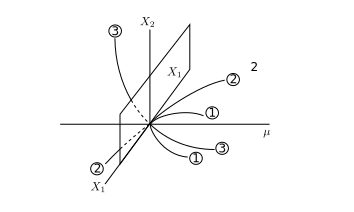
\includegraphics{figure/fig76-2.1.eps}
\caption{}
\end{figure}
\end{example*}

\begin{comment}\label{chap3-com2.2}
The\pageoriginale same picture as above describes the local zero set
of $G$: the only modification consists in replacing the hyperplane
$\{0\} \times X_{1}$ of $\mathbb{R} \times X_{1}$ by the hyperplane
$\{0\} \times X$ in $\mathbb{R} \times X$.
\end{comment}

\begin{center}
{\em THE CASE $k \geq 3$}.
\end{center}

If $k \geq 3$, the mapping (\ref{chap3-eq2.10}) is
\begin{equation*}
D^{2}f(0) \cdot (\mu, x)^{2} = -\frac{2\mu}{\lambda_{0}} Q_{1}x,\tag{2.15}\label{chap3-eq2.15}
\end{equation*}
because $Q_{1}D_{x}^{2}\Gamma(0) = 0$. When $X_{1} \nsubset Y_{2}$
(which can be expected in most of the applications), one has
$D^{2}f(0) \neq 0$ so that the mapping (\ref{chap3-eq2.15}) should
verify the condition $(\mathbb{R}-N.D.)$. Unfortunately, {\em this is
  never the case} when $n \geq 2$ (as assumed throughout this
section). To see this, note that the local zero set of the mapping
(\ref{chap3-eq2.15}) contains the pair $(0, x)$ for any $x \epsilon
X_{1}$. Its derivative at  such a point is given by
$$
(\mu', x') \epsilon \mathbb{R} \times X_{1} \to
-\frac{2\mu'}{\lambda_{0}} Q_{1}x \epsilon Y_{1}.
$$

Its range is the space $\mathbb{R}Q_{1}x$ of dimension $\leq 1$ and it
cannot be onto for $n \geq 2$ (note that it is onto when $n = 1$ and
$X = X_{1} \oplus Y_{2}$ so that there is no contradiction with the
results of Chapter \ref{chap1}).

However, it is possible to overcome the difficulty by performing a {em
change of scale} in our initial problem. The idea is as follows. For
any {\em odd} integer $p$, the mapping
$$
\eta \epsilon \mathbb{R} \to \eta^{\rho} \epsilon \mathbb{R},
$$
is\pageoriginale a $C^{\infty}$ homeomorphism. One can then wonder
whether there is a ``suitable'' choice of the odd integer $\rho \geq 3$
such that, setting $\mu = \eta^{p}$, the results of Chapter
\ref{chap2}, $\S 4$ apply to the problem: Find $(\eta, x)$ around the
origin of $\mathbb{R} \times X$ such that
\begin{equation*}
G(\eta^{p}, x) = (I - (\lambda_{0} + \eta^{p})L)x + \Gamma(\eta^{p},
x) = 0.\tag{2.16}\label{chap3-eq2.16}
\end{equation*}

The Lyapunov-Schmidt reduction of this new problem yields a reduced
equation
$$
g(\eta, x) = 0,
$$
for $(\eta, x)$ around the origin in $\mathbb{R} \times X_{1}$, where
the mapping is easily seen to be
$$
g(\eta, x) = f(\eta^{p}, x),
$$
the mapping $f$ being the reduced mapping in (\ref{chap3-eq2.8}) of the
problem (\ref{chap3-eq2.1}). In particular, the mapping which is found
through the Implict function theorem in the Lyapunov-Schmidt reduction
is exactly $\varphi(\eta^{p}, x)$ where $\varphi$ is characterized by
(\ref{chap3-eq2.9}) and the solutions to the problem
(\ref{chap3-eq2.1}) are the pairs
\begin{equation*}
\{(\eta^{p}, x + \varphi(\eta^{p}, x)) \epsilon \mathbb{R} \times X,
(\eta, x) \epsilon \mathbb{R} \times X_{1}, g(\eta, x) = 0 \}.\tag{2.17}\label{chap3-eq2.17}
\end{equation*}

Intuitively, the choice of $p$ can be made by examinin the function
\begin{equation*}
g(\eta, x) = -\frac{\eta^{p}}{\lambda_{0}} Q_{1}x -
\frac{\eta^{p}}{\lambda_{0}} Q_{1}\varphi (\eta^{p}, x) +
Q_{1}\Gamma(\eta^{p}, x + \varphi(\eta^{p}, x)).\tag{2.18}\label{chap3-eq2.18}
\end{equation*}

As $D\varphi(0) = 0$, the leading term in the expression
$-(\eta^{p} / \lambda_{0})Q_{1} x - (\eta^{p}/\lambda_{0})
Q_{1}\varphi(\eta^{p}, x)$ is $-(\eta^{p}/\lambda_{0})Q_{1}x$. On the
other hand, in\pageoriginale analogy with the case $k = 2$, it might
be desirable that the term $Q_{1}D_{x}^{k}\Gamma(0) \cdot (x)^{k}$ as
well as the first nonzero derivative of the term $- (\eta^{p}/
\lambda_{0})Q_{1}x$ at the origin be in the expression of the first
nonzero derivative of $g$ at the origin. The later is of order $p + 1$
whereas the term $D_{x}^{k}\Gamma(0) \cdot (x)^{k}$ does not appear
before differentiatinf $k$ times. A ``good'' relation thus seems to be $p
+ 1 = k$, namely $p = k - 1$.

This turns out be the right choice of $p$, which can actually be found
after eliminating all the other values on the basis of natural
mathematical requirements instead of using the above intuitive
arguments. Of course, a mathematical method for finding the proper
change of parameter may have some importance in problems in which
there is no a priori guess of what it should be. Incidentally, one can
also provide a complete justification of the use of Newton diagrams in
the change of scale as is done, for instance, in Sattinger
\cite{34}. However, the study is technical and too long to be presented
here (cf. Rabier \cite{31}).

As we have assumed that $p$ is odd for the reasons explained above, we
must suppose that $k$ is even. A similar method will be analysed later
on when $k$ is odd.

{\em The case $k$ even}: We need to find the first nonzero derivative of
the mapping of (\ref{chap3-eq2.18}) at the origin in $\mathbb{R}
\times X_{1}$ when $p = k - 1$. We can already guess that it will be of
order $k$ but we have\pageoriginale to determine its explict expression
in terms of the data. With this aim, we first prove
\begin{lemma}\label{chap3-lem2.1}
Around the origin in $\mathbb{R} \times X$. one has
$$
Q_{1}\Gamma(\eta^{k-1}, x) = \frac{1}{k!} Q_{1}D_{x}^{k}\Gamma(0)
\cdot (x)^{k} + \circ (|\eta| + |||x|||)^{k}),
$$
where $|||\cdot|||$ denote the norm of the space X.
\end{lemma}

\begin{proof}
From the assumption $k \geq 3$, $D\Gamma(0) = 0$ and
$Q_{1}D^{2}\Gamma(0) = 0$, since we already saw that
$D_{\mu}^{2}\Gamma(0) = 0$, $D_{\mu}D_{x}\Gamma(0) = 0$
(cf. (\ref{chap3-eq2.5}) - (\ref{chap3-eq2.6})). Thus, the Taylor
formula about the origin yields
$$
Q_{1}\Gamma(\mu, x) = \sum\limits_{j=3}^{k} \frac{1}{j!}
Q_{1}D^{j}\Gamma(0).(\mu, x)^{j} + 0 (|\mu| + |||x|||)^{k}),
$$
For any $j$ with $3 \leq j \leq k$, one has
$$
Q_{1}D^{j}\Gamma(0)(\mu, x)^{j} = \sum\limits_{i=0}^{j} \binom{j}{i} 
\mu^{j-i} Q_{1}D_{\mu}^{j-i} D_{x}^{i} \Gamma(0) \cdot (x)^{i}.
$$

But, from (\ref{chap3-eq2.5}) $D_{\mu}^{j}\Gamma(0) = 0$ for every $j$
and the index i actually runs over the set $\{1, \cdots, j\}$. Also,
for $j < k$, it follows, from (\ref{chap3-eq2.7}), that $i$ runs over
the set $1, \cdots, j-1$ only. To sum up,
\begin{align*}
Q_{1}\Gamma(\mu, x) &= \frac{1}{k!} Q_{1}D_{x}^{k}\Gamma(0) \cdot
(x)^{k} + \sum\limits_{j=3}^{k} \frac{1}{j!} \sum\limits_{i=1}^{j-1}
(_{i}^{j}) \mu^{j-i} Q_{1}D_{\mu}^{j-i}\\
&\qquad\qquad D_{x}^{i}\Gamma(0) \cdot (x)^{i} + o ((|\mu| + |||x|)^{k}).
\end{align*}

Replacing $\mu$ by $\eta^{k-1}$, we shall see that each term in the
sum is of order $o(|\eta| + |||x|||)^{k})$, except for $(1/k!)
Q_{1}D_{x}^{k}\Gamma(0) \cdot (x)^{k}$. This is obvious as concerns
the remainder which becomes $o ((|\eta|^{k-1} + |||x|||)^{k})$ and, for
$3 \leq j \leq k$ and $1 \leq i \leq j - 1$, each term in the sum is
of order
$$
0(|\eta|^{(k-1)(j-i)} |||x|||^{i}).
$$

Replacing\pageoriginale $|\eta|$ and $||x||$ by $|\eta| + |||x|||$, it
is {\em a fortiori} of order
$$
0 ((|\eta| + |||x|||)^{(k-1)(j-i)+1}).
$$

As $j - i \geq 1$ and $j - i = 1$ if and only if $i = j - 1$, we have,
for $i = j - 1$
$$
(k-1) + (j-1) \geq k+1
$$
ecause $j \geq 3$. On the other hand, if $j-i \geq 2$ and since $i
\geq 1$
$$
(k-1)(j-i) + i \geq 2(k-1) + 1 = 2k - 1 \geq k + 1.
$$

In any case, each term is of order
$$
0((|\eta| + |||x|||)^{k+1}),
$$
which completes the proof.
\end{proof}

\begin{proposition}\label{chap3-prop2.1}
The first nonzero derivative of the mapping
\begin{align*}
(\eta, x) \epsilon \mathbb{R} \times X_{1} \to g(\eta, x) & =
  f(\eta^{k-1}, x) = -\frac{\eta^{k-1}}{\lambda_{0}} Q_{1}x -
  \frac{\eta^{k-1}}{\lambda_{0}} Q_{1}\varphi (\eta^{k-1}, x) \tag{2.19}\label{chap3-eq2.19}\\
& + Q_{1}\Gamma(\eta^{k-1}, x+\varphi(\eta^{k-1}, x)) \epsilon Y_{1}
\end{align*}
at the origin is of order k and its value at the point $(\eta, x)
\epsilon \mathbb{R} \times X_{1}$ repeated k times (which determines
it completely) is
\begin{equation*}
D^{k}g(0) \cdot (\eta, x)^{k} = -\frac{k!}{\lambda_{0}} \eta^{k-1}
Q_{1} x + Q_{1}D_{x}^{k} \Gamma(0) \cdot (x)^{k}.\tag{2.20}\label{chap3-eq2.20}
\end{equation*}
\end{proposition}

\begin{proof}
As $D\varphi(0) = 0$, one has
$$
\varphi(\mu, x) = o(|\mu| + |||x|||),
$$
around\pageoriginale the origin. In particular, replacing $\mu$ by
$\eta^{k-1}$
\begin{equation*}
\varphi(\eta^{k-1}, x) = o(|\eta| + |||x||),\tag{2.21}\label{chap3-eq2.21}
\end{equation*}
so that the term $(\eta^{k-1} / \lambda_{0}) Q_{1}\varphi(\eta^{k-1},
x)$ is of order
\begin{equation*}
(\eta^{k-1}/\lambda_{0})Q_{1}\varphi(\eta^{k-1}, x) = 0(|\eta|^{k-1} o
  (|\eta| + |||x|||)) = o(|\eta| + |||x|||)^{k}).\tag{2.22}\label{chap3-eq2.22}
\end{equation*}

Next, from Lemma \ref{chap3-lem2.1},
\begin{align*}
Q_{1}\Gamma(\eta^{k-1}, x+\varphi(\eta^{k-1}, x)) & = \frac{1}{k!}
Q_{1} D_{x}^{k}\Gamma(0) \cdot (x + \varphi(\eta^{k-1}, x))^{k}\\
& + o((|\eta| + |||x + \varphi (\eta^{k-1},
x)|||)^{k}).\tag{2.23}\label{chap3-eq2.23} 
\end{align*}

But 
$$
|\eta| + |||x+\varphi(\eta^{k-1}, x)||| = 0(|\eta| + |||x||| +
|||\varphi(\eta^{k-1}, x)|||).
$$

Using (\ref{chap3-eq2.21}), we see that
$$
o(|\eta| + |||x||| + |||\varphi(\eta^{k-1}, x)|||) = o(|\eta| +
|||x||| + o(|\eta| + |||x|||)) = o(|\eta| + |||x|||).
$$

Thus, the remainder in (\ref{chap3-eq2.23}) is
$$
o(|\eta| + |||x+\varphi(\eta^{k-1}, x)|||)^{k}) = o([0(|\eta| +
  |||x|||)]^{k}) = o((|\eta| + ||x||)^{k}),
$$
so that
\begin{equation*}
Q_{1}\Gamma(\eta^{k-1}, x+\varphi(\eta^{k-1}, x)) = \frac{1}{k!}
Q_{1}D_{x}^{k}\Gamma(0) \cdot (x + \varphi(\eta^{k-1}, x))^{k} +
o((|\eta| + |||x|||)^{k}).\tag{2.24}\label{chap3-eq2.24}
\end{equation*}

Now, from (\ref{chap3-eq2.21}) again and due to the $k$-linearity of the
derivative $D_{x}^{k}\Gamma(0)$, we deduce
$$
Q_{1}D_{x}^{k}\Gamma(0) \cdot (x+\varphi(\eta^{k-1}, x))^{k} =
Q_{1}D_{x}^{k}\Gamma(0) \cdot (x)^{k} + o(|\eta| + |||x||)^{k}).
$$

By putting this expression in (\ref{chap3-eq2.24}) and together with
(\ref{chap3-eq2.22}), the mapping\pageoriginale $g$ (\ref{chap3-eq2.19})
can be rewritten as
\begin{equation*}
g(\eta, x) = -\frac{\eta^{k-1}}{\lambda_{0}} Q_{1}x +
\frac{1}{k!}Q_{1}D_{x}^{k}\Gamma(0) \cdot (x)^{k} + o((|\eta| +
|||x|||)^{k}).\tag{2.25}\label{chap3-eq2.25} 
\end{equation*}

This relation shows that the first $k - 1$ derivatives of $g$ vanish at
the origin. Besides, from Taylor's formula, we have
$$
g(\eta, x) = \frac{1}{k!} D^{k}g(0) \cdot (\eta, x)^{k} + o(|\eta| +
|||x|||)^{k}), 
$$
which, on comparing with (\ref{chap3-eq2.25}), yields
$$
D^{k}g(0) \cdot (\eta, x)^{k} = -\frac{k!}{\lambda_{0}} \eta^{k-1}
Q_{1}x + Q_{1}D_{x}^{k}\Gamma(0) \cdot (x)^{k}.
$$
\end{proof}

\begin{remark}\label{chap3-rem2.3}
We leave it to the reader to check that {\em the same result holds} if
we replace conditions (\ref{chap3-eq2.7}) by
\begin{align*}
& D_{x}^{j}\Gamma(0) |_{(X_{1})j} = 0, 0 \leq j \leq k-1,\\
& Q_{1}D_{x}^{k}\Gamma(0) |_{(X_{1})^{k}} \neq 0.\tag{2.26}\label{chap3-eq2.26}
\end{align*}

More generally, it still holds under {\em some combination} of the
hypotheses (\ref{chap3-eq2.7}) and (\ref{chap3-eq2.26}): Denoting by
$k$ the order of the first non-zero derivative with respect to $x$ of the
mapping $Q_{1}\Gamma |_{\mathbb{R} \times X_{1}}$ at the origin
(suppose to be finite), set
\begin{align*}
k_{1} & = \min \{0 \leq j \leq k, Q_{1}D_{x}^{j}\Gamma(0) \neq 0 \},\tag{2.27}\label{chap3-eq2.27}\\
k^{1} & = \min \{0 \leq j \leq k, D_{x}^{j}\Gamma(0) |_{(X_{1})j} \neq
0\},\tag{2.28}\label{chap3-eq2.28}\\
\end{align*}
so\pageoriginale that $2 \leq k_{1}, k^{1} \leq k$. Then, it can be
shown (cf. \cite{31}) that Proposition 2.7 remains true when
\begin{equation*}
k \leq k_{1} + k^{1} - 2.\tag{2.29}\label{chap3-eq2.29}
\end{equation*}

Note that $k = k_{1}$ in our assumptions whereas $k = k^{1}$ under the
hypotheses (\ref{chap3-eq2.26}), two cases when the criterion
(\ref{chap3-eq2.29}) is satisfied.
\end{remark}

When the mapping $D^{k}g(0) \cdot (\eta, x)^{k}$ in
(\ref{chap3-eq2.20}) verifies the condition $(\mathbb{R}-N.D.)$, the
results of Chapter \ref{chap2}, $\S 4$ give the structure of the local
zero set of $g$ (\ref{chap3-eq2.19}). We shall derive the structure of
the local zero set of f but, first observe that

\begin{proposition}\label{chap3-prop2.2}
The mapping $D^{k}g(0) \cdot (\eta, x)^{k}$ in (\ref{chap3-eq2.20})
can verify the condition $(\mathbb{R}-N.D.)$ only if the following two
implict conditions are fulfilled:
\begin{enumerate}
\item[(i)] $X = X_{1} \oplus Y_{2} (= Ker (I - \lambda_{0} L) \oplus
  Range (I - \lambda_{0} L))$\footnote{Namely, the algebraic
    muliplicity of $\lambda_{0}$ equals its geometric multiplicity.},

\item[(ii)] $Q_{1}D_{x}^{k}\Gamma(0) \cdot (x)^{k} \neq 0$ {\em for
  every} $x \epsilon X_{1} - \{0\}$.
\end{enumerate}
\end{proposition}

\begin{proof}
(i) Assume thatg $X_{1} \cap Y_{2} = \{0\}$. The trivial branch
  $\{(\eta, 0); \eta \epsilon \mathbb{R}\}$ is in the zero set
  $D^{k}g(0) \cdot (\eta, x)^{k}$ and its derivative at any of its
  nonzero points is
$$
(\eta', x') \epsilon \mathbb{R} \times X_{1} \to -
  \frac{k!}{\lambda_{0}} \eta^{k-1} Q_{1} x' \epsilon Y_{1},
$$
whose range is Range $Q_{1} |_{X_{1}} \subsetneq Y_{1}$ since Ker
$Q_{1} |_{X_{1}} \neq \{0\}$ from the assumption\pageoriginale $X_{1}
\cap Y_{2} \neq \{0\}$.

(ii) Assume there is a nonzero $x \epsilon X_{1}$ such that
$Q_{1}D_{x}^{k}\Gamma(0) \cdot (x)^{k} = 0$. Then, the line
$\mathbb{R}(0, x)$ is in the zero set of $Q_{1}D^{k}g(0) \cdot (\eta,
x)^{k}$ and its derivative at $(0, x)$ is 
$$
(\eta', x') \epsilon \mathbb{R} \times X_{1} \to
kQ_{1}D_{x}^{k}\Gamma(0) \cdot (x^{k-1}, x') \epsilon Y_{1},
$$
whose null-space contains the trivial branch and the line
$\mathbb{R}(0, x)$ : its range is then at most $(n-1)$-dimensional.
\end{proof}

\begin{comment}\label{chap3-com2.3}
Assume that the mapping $D^{k}g(0) \cdot (\eta, x)^{k}$
(\ref{chap3-eq1.20}) verifies the condition $(\mathbb{R}-N.D.)$. From
our analysis of $\S 1$, this assumption is {\em independent of the
  choice of the complements} $X_{2}$ and $Y_{1}$ of $X_{1}$ and
$Y_{2}$ respectively. In the applications, it follows from Proposition
\ref{chap3-prop2.2} that we can take $X_{1} = Y_{1}$ so that the
mapping $g$ becomes (note that $Q_{1}\varphi = 0$ in this case)
\begin{equation*}
g(\eta, x) = -\frac{\eta^{k-1}}{\lambda_{0}} x +
Q_{1}\Gamma(\eta^{k-1}, x + \varphi(\eta^{k-1}, x))\tag{2.30}\label{chap3-eq2.30}
\end{equation*}
and one has
\begin{equation*}
D^{k}g(0) \cdot (\eta, x)^{k} = -k! \frac{\eta^{k-1}}{\lambda_{0}} x +
Q_{1}D_{x}^{k}\Gamma(0) \cdot (x)^{k},
\end{equation*}
for every $(\eta, x) \epsilon \mathbb{R} \times X_{1}$.
\end{comment}

\begin{comment}\label{chap3-com2.4}
From (ii) of Proposition \ref{chap3-eq2.2}, none of the lines of the
zero set of $D^{k}g(0) \cdot (\eta, x)^{k}$ is ``vertical'' i.e. lies
on the hyperplane $\{0\} \times X_{1}$ of $\mathbb{R} \times
X_{1}$. In other words, if $t \to (\eta(t), x(t))$ is any
curve\pageoriginale in the local zero set of $g$, one has
\begin{equation*}
\frac{d\eta}{dt} (0) \neq 0.\tag{2.32}\label{chap3-eq2.32}
\end{equation*}
\end{comment}

\begin{comment}\label{chap3-com2.5}
The trivial branch is in the zero set of the mapping $D^{k}g(0) \cdot
(\eta, x)^{k}$ (and {\em also} in the local zero set of $g$ since
$\varphi(\mu, 0) = 0$; cf. Chapter \ref{chap1}). As $k$ is even, we know
that the number $\nu$ of lines must be evern too $(\leq k^{n})$. Thus
$\nu \geq 2$ and {\em bifurcation occurs} (as in the case $k = 2$). In
view (\ref{chap3-eq2.32}), each curve is located on both sides of the
hyperplane $\{0\} \times X_{1}$ (i.e. bifurcation occurs {\em
  transcritically}).
\begin{figure}[H]
\centering
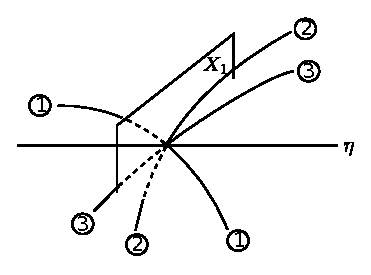
\includegraphics{figure/fig76-2.2.eps}
\caption{Local zero set of $g$.}
\end{figure}
\end{comment}

We now pass to the description of the local zero set of $f$: it is made
up of the $\nu$ curves
\begin{equation*}
t \to (\mu(t), x(t)),\tag{2.33}\label{chap3-eq2.33}
\end{equation*}
where\pageoriginale $\mu(t) = \eta^{k-1}(t)$ and $t \to (\eta(t),
x(t))$ is one of the $\nu$ curves in the local zero set of $g$, hence of class
$C^{m-k+1}$ at the origin and of class $C^{m}$ away from it. Of
course, the $\nu$ curves in (\ref{chap3-eq2.33}) are {\em distinct}
sicne the mapping $\eta \to \eta^{k-1}$ is a homeomorphism. Also, it
is clear that $(d\mu/dt)(0) = 0$ so that
\begin{equation*}
\frac{d}{dt} (\mu(t), x(t)) |_{t=0} = (0, \frac{dx}{dt} (0)).\tag{2.34}\label{chap3-eq2.34}
\end{equation*}

But, for each curve $(\eta(t), x(t))$ in the local zero set of $g$ which
is {\em distinct from the trivial branch}, we must have
$$
\frac{dx}{dt}(0) \neq 0,
$$
because different curves in the local zero set of $g$ have different
tangents at the origin. Thus, for each curve $(\mu(t), x(t))$ in the
local zero set of $f$ which is {\em distinct from the trivial branch},
one has 
$$
\frac{d}{dt} (\mu(t), x(t)) |_{t=0} = (0, \frac{dx}{dt} (0)) \neq 0.
$$

As a result and further since the functions $\mu(t) = \eta^{k-1}(t)$
and $x(t)$ are of class $C^{m-k+1}$ at the origin and of class $C^{m}$
away from it, we may deduce that the nontrivial curves in the local
zero set of $f$ are also of class $C^{m-k+1}$ at the origin and of class
$C^{m}$ away from it. Besides, due to (\ref{chap3-eq2.34}), {\em they
  are tangent to the hyperplane} $\{0\} \times X_{1}$ of $\mathbb{R}
\times X_{1}$ at the origin. Finally, as the sign of $\mu(t) =
\eta^{k-1}(t)$ changes as that $\eta(t)$ does, bifurction remains
transcritical (cf. Comment \ref{chap3-com2.5}) as in the case when $k
= 2$ and the condition $Q_{1}D_{x}^{2}\Gamma(0) \cdot (x) \neq 0$ for
every\pageoriginale $x \epsilon X_{1} - \{0\}$ holds (cf. Comment
\ref{chap3-com2.1})\footnote{Recall however that this condition is not
required when $k = 2$.}.
\begin{figure}[H]
\centering
\includegraphics{figure/fig76-2.3.eps}
\caption{Local zero set of $f$ ($k$ even)}
\end{figure}


\begin{remark}\label{chap3-rem2.4}
It is possible for several curves in the local zero set of $f$ to have
the {\em same} tangent at the origin: This will happen if and only if
several lines in the zero set of the mapping $D^{k}g(0) \cdot (\eta,
x)^{k}$ (\ref{chap3-eq2.20}) have the same projection onto $X_{1}$
(along the $\eta$-axis). If this is the case, that is one more reason
for the assumptions of Chapter \ref{chap2}, $\S 4$ to fail when the
parameter $\mu$ is unchanged, for, when the curves are found through
Theorem \ref{chap2-thm4.1} of Chapter \ref{chap2}, they must have {\em
different tangents at the origin}.
\end{remark}

{\em The case $k$ odd}: When $k$ is odd, the mappping $\eta \to
\eta^{k-1}$ is\pageoriginale no longer a homeomorphism. However, by
performing the change $\mu = \eta^{k-1}$, we shall find all solutions
in the local zero set of f associated with $\mu \geq 0$. In order to
get the solutions associted with $\mu \leq 0$, it suffices to perform
the change $\mu = -\eta^{k-1}$.

The method is quite similar and we shall set
\begin{align*}
g_{\sigma}(\eta, x) = f(\sigma \eta^{k-1}, x) & = - \frac{\sigma
  \eta^{k-1}}{\lambda_{0}} Q_{1}x - \frac{\sigma
  \eta^{k-1}}{\lambda_{0}} Q_{1}\varphi(\sigma \eta^{k-1}, x) +\\
& + Q_{1}\Gamma(\sigma \eta^{k-1}, x + \varphi(\sigma \eta^{k-1}, x)),\tag{2.35}\label{chap3-eq2.35}
\end{align*}
where $\sigma = \pm 1$. Arguing as in Proposition \ref{chap3-prop2.1},
we find that the first nonzero derivative of the mapping $g_{\sigma}$
at the origin is of order $k$ with
\begin{equation*}
D^{k}g_{\sigma}(0) \cdot (\eta, x)^{k} = - \frac{\sigma
  k!}{\lambda_{0}} \eta^{k-1} Q_{1} x + Q_{1}D_{x}^{k}\Gamma(0) \cdot
(x)^{k} \epsilon Y_{1},\tag{2.36}\label{chap3-eq2.36}
\end{equation*}
for every $(\eta, x) \epsilon \mathbb{R} \times X_{1}$. Again, two
implict condition for the results of Chapter \ref{chap2}, $\S 4$ to be
available are
$$
X = Ker (I - \lambda_{0}L) \oplus Range (I - \lambda_{0}L)(= X_{1}
\oplus Y_{2}),
$$
(i.e. the algebraic and geometric multiplicities of the
characteristic value of $\lambda_{0}$ coincide) and
$$
Q_{1}D_{x}^{k} \Gamma(0) \cdot (x)^{k} \neq 0 \text{ for every } x
\epsilon X_{1} - \{0\}.
$$

Again, from $\S 1$ the mapping $D^{k}g(0)(\eta, x)^{k}$ verifies the
condition $(\mathbb{R}-N.D)$ or not independently of the choice of
$X_{2}$ and $Y_{1}$ so that we can take $X_{1} = Y_{1}$ in the
applications. With this choice, we get the\pageoriginale simplified
expressions
\begin{align*}
& g_{\sigma}(\eta, x) = -\frac{\sigma \eta^{k-1}}{\lambda_{0}} x +
Q_{1}\Gamma (\sigma \eta^{k-1}, x + \varphi (\sigma \eta^{k-1},
x)),\tag*{(2.37)$_{\sigma}$}\label{chap3-eq2.37}\\
& D^{k}g_{\sigma}(0) \cdot (\eta, x)^{k} = -\frac{\sigma k!
  \eta^{k-1}}{\lambda_{0}} x + Q_{1}D_{x}^{k}\Gamma(0) \cdot (x)^{k}
\epsilon X_{1},\tag*{(2.38)$_{\sigma}$}\label{chap3-eq2.38}
\end{align*}
for every $(\eta, x) \epsilon \mathbb{R} \times X_{1}$. Also, none of
the curves in the local zero set of $g_{\sigma}$ has a ``vertical''
tangent at the origin and each curve in the local zero set of $f$ is of
the from
$$
t \to (\mu(t), x(t)),
$$
with $\mu(t) = \sigma \eta^{k-1}(t)$ and $t \to (\eta(t), x(t))$ is
one of the curves in the local zero set of $g_{\sigma}$ (thus of class
$C^{m-k+1}$ at the origin and of class $C^{m}$ away from it). Each
non-trivial curve in the local zero set of $f$ is then also of class
$C^{m-k+1}$ at the origin and of class $C^{m}$ away from it (the
argument is the same as when $k$ is even) and it is tangent to the
hyperplane $\{0\} \times X_{1}$ at the origin. For $\sigma = 1$
(respectively - 1), the corresponding curves of the local zero set of
$f$ are located in the half space $\mu \geq 0$ (respectively $\mu \leq
0$) because, contrary to what happens when $k$ is even, $\sigma
\eta^{k-1}(t)$ {\em does not} change sign here.
\begin{figure}[H]
\centering
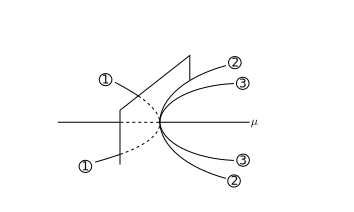
\includegraphics{figure/fig76-2.4.eps}
\caption{Local zero set of $f$ ($k$ odd).}
\end{figure}

The\pageoriginale differences with the case when $k$ is even are as
follows: (i) Both mapping \ref{chap3-eq2.38} must verify the
condition $(\mathbb{R}-N.D.)$ for $\sigma = 1$ and $\sigma =
-1$. Charging $\eta$ into $e^{i \pi (k-1)} \eta$, it is easy to see
that this is the case if one of them verifies the condition
$(\mathbb{C}-N.D.)$, because this property is invariant under
$\mathbb{C}$-linear changes of variables.

(ii) Bifurcation (i.e. existence of notrivial curves) is {\em not
  ensured} (an example was given in Chapter \ref{chap1}). However,
bifurcation occurs if $\eta$ is odd (Theorem \ref{chap1-thm1.2} of
Chapter \ref{chap1}). This means that for at least one of the values
$\sigma = 1$ or $\sigma = -1$, the zero set of the mapping
$D^{k}g_{\sigma}(0) \cdot (\eta, x)^{k}$ contains at least one
nontrivial line.

\begin{remark}\label{chap3-rem2.5}
Theorem \ref{chap1-thm1.2} of Chapter \ref{chap1} (Krasnoselskii's
theorem) is based\pageoriginale on topological degree arguments. Is
there however a purely algebraic proof of the above statement?
\end{remark}

(iii) Let $\nu_{\sigma}, \sigma = \pm 1$ denote the number of curves
in the local zero set of the mapping $g_{\sigma}$. Then, {\em a
  priori}, the number of curves in the local zero set of $f$ is $\nu_{1}
+ \nu_{-1}$. Actually, $\nu_{1}$ and $\nu_{-1}$ must be {\em odd} and
the number of {\em distinct} curves in the local zero set of $f$ is
$(\nu_{1} + \nu_{-1} )/ 2$ (hence $\leq k^{n}$ again since
  $\nu_{\sigma} \leq k^{n}$). Indeed, it is clear from the evenness of
  $k - 1$ that when a curve $(\eta(t), x(t))$ is in the local zero set
  of $g_{\sigma}$, the curve $(-\eta(t), x(t))$ is also in it. Both
  provide the same curve $(\mu(t), x (t)) = (\sigma \eta^{k-1}(t),
  x(t))$ in th local zero set of $f$ and the two vectors $((d\eta/dt)(0)
  (dx/dt)(0))$ and $(-(d\eta/dt)(0), (dx/dt)(0))$ are not collinear if
  and only if $(dx/dt)(0)\neq 0$, because $(d\eta/dt)(0)$ is $\neq 0$
  as we observed earlier\footnote{In comment \ref{chap3-com2.4} and
    when $k$ is even, but the argument can be repeated when $k$ is
    odd.}. Now the condition $(dx/dt)(0) \neq 0$ is fulfilled by all
  the curves in the local zero set of $g_{\sigma}$, except the trivial
  branch (recall that the correspondence between the curves in the
  local zero set of $g_{\sigma}$ and their tangents at the origin is
  one-to-one). Hence, each non-trivialcurve in the local zero set of $f$
  is provided by {\em two} distinct non-trivial curves in the local
  zero set of $g_{1}$ or by two distinct non-trivial curves in the
  local zero set of $g_{-1}$. Thus, $\nu_{1}$ and $\nu_{-1}$ must be
  odd and the number of non-trivial curves in the local zero set of $f$
  is
$$ 
\frac{\nu_{1} - 1}{2} + \frac{\nu_{-1}-1}{2} = \frac{\nu_{1} +
  \nu_{-1}}{2}  -1. 
$$

Adding\pageoriginale the trivial branch, we find $(\nu_{1} + \nu_{-1})
|2$ to be the number of distinct curves in the local set of $f$. Exactly
$(\nu_{1} - 1)| 2$ of them are supercritical (i.e. located in the
half-space $\mu \geq 0$ of $\mathbb{R} \times X_{1}$) and exactly
$(\nu_{-1} - 1) | 2$ are subcritical (i.e. located in the half space
$\mu \leq 0$ of $\mathbb{R} \times X_{1}$). One (the trivial branch)
is {\em transcritical}. Of course, it may happen that $\nu_{1} = 0$ or
$\nu_{-1} = 0$ (or both).

\begin{remark}\label{chap3-rem2.6}
Recall that in both the case ($k$ {\em even} and $k$ {\em odd}), we made
the {\em a priori} assumption $X_{1} \nsubset Y_{2}$ (and it turned
out that the conditions $X_{1} \cap Y_{2} = \{0\}$ was necessary). If
$X_{1} \subset Y_{2}$, the trick of changing the parameter $\mu$ into
$\eta^{k-1}$, $\sigma = \pm 1$ does not work: Indeed, the first
nonzero derivative of $g$ or $g_{\sigma}$ at the origin remains of order
$k$ and its value at the point $(\eta, x) \epsilon \mathbb{R} \times
X_{1}$ repeated $k$ times reduces to
$$
(\eta, x) \epsilon \mathbb{R} \times X_{1} \to Q_{1}D_{x}^{k}\Gamma(0)
\cdot (x)^{k} \epsilon Y_{1}.
$$

This mapping {\em never verifies the condition} $(\mathbb{R}-N.D.)$ because
of the trivial branch in its zero set at which its derivative vanishes.
\end{remark}

\begin{remark}\label{chap3-rem2.7}
We leave it to the reader to check that changing the paramete $\mu$
into $a$ $\eta^{k-1}$, $a \neq 0$, when $k$ is even is equivalent to
changing it into $\eta^{k-1}$ (i.e. $a = 1$) as we have done. No more
generality will be reached either by changing $\mu$ into $a$ $\eta^{k-1}
+ o(\eta^{k-1})$, $a \neq 0$ and\pageoriginale {\em no other exponent}
$p \neq k-1$ can be used in the change $\mu = \eta^{p}$ (because the
condition $(\mathbb{R}-N.D.)$ always fails with such a
choice). Similarly, when $k$ is {\em odd}, changing $\mu$ into
$a \eta^{k-l} + \circ (\eta^{k-l})$, $a>0$ is equivalent to changing $\mu$ into $\eta^{k-l}$ and changing $\mu$ into $a \eta^{k-1} + o(\eta^{k-1})$
is equivalent to changing $\mu$ into $-\eta^{k-1}$ 
\end{remark}

To complete this section, we come back to the case $n = 1$ for
comparisons and further comments. In Chapter \ref{chap1}, we have
solves the problem without any assumption on the derivatives
$Q_{1}D_{x}^{j}\Gamma(0) |_{(X_{1})^j}$ and the condition
$(\mathbb{R}-N.D.)$ was seen to be equivalent to the fact that the
algebraic multiplicity of $\lambda_{0}$ equals its geometric
multiplicity i.e. 
\begin{equation*}
X = Ker (I - \lambda_{0}L) \oplus Range (I - \lambda_{0}L)(= X_{1}
\oplus Y_{2}).\tag{2.39}\label{chap3-eq2.39}
\end{equation*}

Neverthless, if there is an integer $3 \leq k \leq m$\footnote{If $k =
  2$, see Comment \ref{chap3-com2.1}.} such that
\begin{align*}
& Q_{1}D_{x}^{j}\Gamma(0) = 0, 0 \leq j \leq k-1,\\
& Q_{1}D_{x}^{k}\Gamma(0) |_{(X_{1})^{k}} \neq 0,\tag{2.40}\label{chap3-eq2.40}
\end{align*}
the trick of changing the parameter $\mu$ into $\eta^{k-1}$ ($k$ even)
or $\sigma \eta^{k-1}$, $\sigma = \pm 1$ ($k$ odd) works as when $n$ is
$\geq 2$ and the analysis we have made in this section can be repeated
with no modification. In particular, condition (\ref{chap3-eq2.39})
remains necessary. Here, it is also a\pageoriginale sufficient
condition for the mapping $D^{k}g(0) \cdot (\eta, x)^{k}$
(\ref{chap3-eq2.20}) (or $D^{k}g_{\sigma}(0) \cdot (\eta, x)^{k}$
(\ref{chap3-eq2.38})) to verify the condition
$(\mathbb{R}-N.D.)$. Indeed, as $X_{1}$ and $Y_{1}$ are
one-dimensional, we can write $x \epsilon X_{1}$ in the form
$$
x = tx^{0}, 
$$
for some $t \epsilon \mathbb{R}$, where $x^{0}$ is a given non-zero
element of $X_{1}$. Also let $y^{0}$ be a given non-zero element of
$Y_{1}$\footnote{From (\ref{chap3-eq2.39}), the choice $x^{0} = y^{0}$
is available and brings slight simplifications in the formulae.} and
consider the linear continuous form $y^{*} \epsilon X'(= Y')$
characterized by (cf. Chapter \ref{chap1}, $\S 3$)
\begin{equation*}
\begin{cases}
\langle y^{*}, y^{0} \rangle  = 1,\\
\langle y^{*}, y \rangle  = 0 \text{ for every } y \epsilon Y_{2}.
\end{cases}
\end{equation*}

This linear form allows us to express the projection operator $Q_{1}$
onto the space $Y_{1}$. More precisely
$$
Q_{1}y = \langle y^{*}, y \rangle y^{0},
$$
for every $y \epsilon X(= Y)$. Then, for $k$ {\em even}, we find from
(\ref{chap3-eq2.20}) that 
$$ 
D^{k}g(0) \cdot (\eta, x)^{k} = \left[-\frac{k!
     \eta^{k-1}}{\lambda_{0}} \langle y^{*}, x^{0} \rangle  + t^{k} \langle y^{*},
  D_{x}^{k}\Gamma(0) \cdot (x^{0})^{k} \rangle \right]y^{0}
$$
and proving that this mapping verifies the condition
$(\mathbb{R}-N.D.)$ amounts to proving that the real-valued mapping of
the two real variables $\eta, t$ given by
$$ 
(\eta, t) \epsilon \mathbb{R}^{2} \to - \frac{k!
  \eta^{k-1}}{\lambda_{0}} \langle y^{*}, x^{0}\rangle  + t^{k} \langle y^{*},
D_{x}^{k}\Gamma(0) \cdot (x^{0})^{k} \rangle  \epsilon \mathbb{R},
$$
does\pageoriginale the same, which is {\em always} the case because of
the relations $\langle y^{*},\break x^{0} \rangle  \neq 0$ (since $X_{1} \cap Y_{2} =
\{0\}$) and $\langle y^{*}, D_{x}^{k}\Gamma(0) \cdot (x^{0})^{k} \rangle  \neq 0$
(since $Q_{1}D_{x}^{k}\Gamma(0) |_{(X_{1})^{k}} \neq 0$). Besides, as
expected, the zero set of $D^{k}g(0) \cdot (\eta, x)^{k}$ is the union
of the trivial branch and exactly {\em one nontrivial line}, namely
that line for which
$$ 
t = \left[k! \frac{\langle y^{*}, D_{x}^{k}\Gamma(0) \cdot
    (x^{0})^{k} \rangle }{\lambda_{0} \langle y^{*}, x^{0} \rangle }\right]^{1/k-1} \eta,
\eta \epsilon \mathbb{R}.
$$

Repeating the arguments we used in the case $n \geq 2$, we see that
the corresponding non-trivial branch in the local ero set of is
tangent to the asis $\{0\} \times X_{1}$ at the origin and located on
both sides of it: we are in the presence of a phenomenon of {\em
  transcritical bifurcation.}
\begin{figure}[H]
\centering
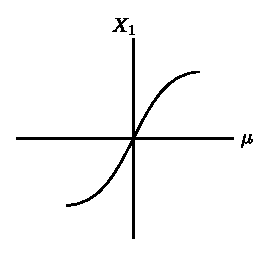
\includegraphics{figure/fig76-2.5.eps}
\caption{Local zero set of $f$ when $n=1$, $k$ even $\geq 4$}
\end{figure}

Analogously, when $k$ is odd, one has (cf. (\ref{chap3-eq2.38}))
$$
D^{k}g_{\sigma}(0) \cdot (\eta, x)^{k} = \left[-k! \frac{\sigma
    \eta^{k-1} t}{\lambda_{0}} \langle y^{*}, x^{0} \rangle  + t^{k} \langle y^{*},
  D_{x}^{k}\Gamma(0) \cdot (x^{0})^{k} \rangle \right]y^{0}.
$$

If\pageoriginale so, because $k-1$ is even, the local zero set of this
mapping {\em reduces to the trivial branch} if
$$
sgn \left[\frac{ \langle y^{*}, 
    D_{x}^{k}\Gamma(0)\cdot(x^{0})^{k} \rangle }{\lambda_{0} \langle y^{*},
    x^{0} \rangle }\right] = sgn (-\sigma)
$$ 
and is the union of the trivial branch and {\em two} nontrivial lines,
namely, those for which 
$$
t = \pm \left[k! \sigma \frac{\langle y^{*}, D_{x}^{k}\Gamma(0) \cdot
    (x^{0})^{k} \rangle}{\lambda_{0} \langle y^{*}, x_{0} \rangle}\right]^{1/k - 1} \eta,
\eta \epsilon \mathbb{R},
$$
if 
$$
sgn \left[\frac{\langle y^{*}, D_{x}^{k}\Gamma(0)
   \cdot(x^{0})^{k} \rangle }{\lambda_{0} \langle y^{*}, x^{0} \rangle }\right] = sgn \sigma.
$$

They both provide the {\em same} curve in the local zero set of $f$,
located on one side of the axis $\{0\} \times X_{1}$. The bifurcation
is either {\em supercritical} or {\em subcritical} depending on which
among the mappings $D^{k}g_{1}(0) \cdot (\eta, x)^{k}$ and
$D^{k}g_{-1}(0) \cdot (\eta, x)^{k}$ possesses the non-trivial lines
in its zero set
\begin{figure}[H]
\centering
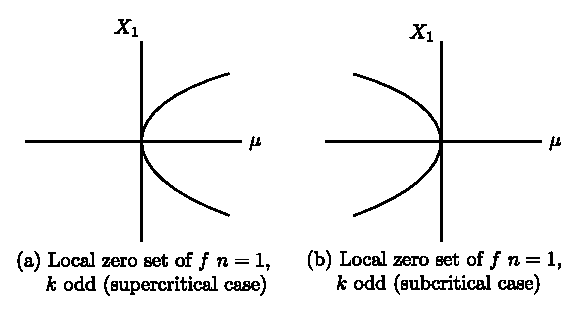
\includegraphics{figure/fig76-2.6.eps}
\caption{}
\end{figure}



\begin{remark}\label{chap3-rem2.8}
Though\pageoriginale the assumptions of this section are stronger than
those we made in Chapter \ref{chap1} when $n = 1$, the regularity of
the non-trivial curve in the local zero set of $f$ is only found to be
of class $C^{m-k+1}$ at the origin (but we know it is actually of
class $C^{m-1}$). In contrast, the location of this curve with respect
to the axis $\{0\} \times X_{1}$ could not be derived from the
analysis of Chapter \ref{chap1} because it clearly depends on the
evenness of $k$, which was ignored in Chapter \ref{chap1}.
\end{remark}

\begin{remark}\label{chap3-rem2.9}
The assumption (\ref{chap3-eq2.40}) can be replaced by 
\begin{align*}
& D_{x}^{j}\Gamma(0) |_{(X_{1})j} = 0, 0 \leq j \leq k-1,\\
& Q_{1}D_{x}^{k}\Gamma(0) |_{(X_{1})^{k}} \neq 0,\tag{2.41}\label{chap3-eq2.41}
\end{align*}
or by a suitable combination (\ref{chap3-eq2.40}) and
(\ref{chap3-eq2.41}) such as in Remark \ref{chap3-rem2.3}.
\end{remark}

\section[Application to a Problem......]{Application to a Problem with
  no Branch of\hfil\break Solutions Known a   Priori.}\label{chap3-sec3} 

We shall here consider the problem of finding the ``small'' solution
$(\mu,\break x) \epsilon \mathbb{R} \times X$ an equation of the form 
\begin{equation*}
F(x) = \mu y^{0}\tag{3.1}\label{chap3-eq3.1}
\end{equation*}
where $F$ is a mapping of class $C^{m}, m \geq 1$, in a neighbourhood of
the origin in the Banach space $X$, with values in another Banch space $Y$,
such that $F(0) = 0$ and where $y^{0}$ is a given element of $Y$. In
order to\pageoriginale deal with a situation essentially different
from that of $\S 2$ we shall assume
\begin{equation*}
y^{0} \notin Range D_{x}F(0).\tag{3.2}\label{chap3-eq3.2}
\end{equation*}

First, we write the problem in the form
$$
G(\mu, x) = 0,
$$
with
\begin{equation*}
G(\mu, x) = F(x) - \mu y^{0}.\tag{3.3}\label{chap3-eq3.3}
\end{equation*}

Due to (\ref{chap3-eq3.2}), the space $Y_{2} = Range DG(0)$ is
\begin{equation*}
Y_{2} = Range DG(0) = \mathbb{R} y^{0} \oplus Range D_{x}F(0)\tag{3.4}\label{chap3-eq3.4}
\end{equation*}
whereas, setting
\begin{equation*}
X_{1} = Ker D_{x}F(0),
\end{equation*}
one has
\begin{equation*}
\widetilde{X}_{1} = Ker DG(0) = \{0\} \times X_{1}.\tag{3.6}\label{chap3-eq3.6}
\end{equation*}

As required in these notes, we shall assume that $DG(0) \epsilon
\mathscr{L} (\mathbb{R} \times X, Y)$ is a Fredholm operator with
index 1, which will be for instance, the case, if $D_{x}F(0)$ is a
Fredholm operator with index 0. As usual, $n$ will denote the codimension
of the space $Y_{2}$.

When $n = 0$, the same problem has already been encountered in Chapter
\ref{chap1}. The situation was simple because the Implict function
theorem applied so that the local zero set of $G$ was found to be made
up\pageoriginale of exactly one curve of class $C^{m}$. Recall that
this curve has a ``vertical'' tangent (i.e. the one - dimensional
space $\{0\} \times X_{1}$) at the origin and we mentioned that two
typical cases where those when the origin is either a {\em ``turning
  point''} or a {\em ``hysteresis point''} (cf. Fig. 3.2 of Chapter
\ref{chap1}). A detailed explanation of these phenomena will be given
later on. For the time being, we shall assume $n \geq 1$. Performing
the Lyapunov-Schmidt reduction as described in Chapter \ref{chap1},
$\S 2$ and setting $\widetilde{x} = (\mu, x)$, we get a reduced
equation of the general form 
$$
f(\widetilde{x}) = Q_{1}G(\widetilde{x} + \widetilde{\varphi}(\widetilde{x})),
$$
where $\widetilde{x}$ belongs to some neighbourhood of the origin in
the space $\widetilde{X}_{1}$ and $Q_{1}$ denotes the projection
operator onto some given complement of the space $Y_{2}$. Because of
(\ref{chap3-eq3.6}), the variable $\widetilde{x} \epsilon
\widetilde{X}_{1}$ identifies itself with the variable $x \epsilon
X_{1}$. Provided we choose the complement $\widetilde{X}_{2}$ of the
space $\widetilde{X}_{1}$ of the form
$$
\widetilde{X}_{2} = \mathbb{R} \times X_{2},
$$
where $X_{2}$ is a given topological complement of $X_{1}$, the
mapping $\widetilde{\varphi}$ can be identified with a pair
$$
\widetilde{\varphi}(x) = (\mu(x), \varphi(x)) \epsilon \mathbb{R}
\times X_{2},
$$
of mappings of class $C^{m}$ aroun the origin.

As $Q_{1}y^{0} = 0$ (cf. (\ref{chap3-eq3.4})), the reduced equation
takes the form 
\begin{equation*}
f(x) = Q_{1}F(x + \varphi(x)) = 0.\tag{3.7}\label{chap3-eq3.7}
\end{equation*}

The\pageoriginale results of Chapter \ref{chap2}, $\S 4$ will be
available if the first nonzero derivative of the above mapping at the
origin verifies the condition $(\mathbb{R}-N.D.)$. A general frame
work in which it takes a very simple expression is as follows:
Consider the integer $2 \leq k \leq m$ characteried by
\begin{equation*}
\begin{cases}
& Q_{1}D_{x}^{j}F(0) |_{(X_{1})j} = 0, 0 \leq j \leq k-1,\\
& Q_{1}D_{x}^{k}F(0) |_{(X_{1})^{k}} \neq 0,
\end{cases}\tag{3.8}\label{chap3-eq3.8}
\end{equation*}
(if such a $k$ exists of course) and let $k_{1}$ and $k^{1}$ be defined
by 
\begin{align*}
k_{1} & = \min \{0 \leq j \leq k, Q_{1}D_{x}^{j}F(0) \neq 0\}, \tag{3.9}\label{chap3-eq3.9}\\
k^{1} & = \min \{0 \leq j \leq k, D_{x}^{j}F(0) |_{(X_{1})^{j}} \neq 0\},\tag{3.10}\label{chap3-eq3.10}
\end{align*}
so that $2 \leq k_{1}, k^{1} \leq k$. Under the
condition\footnote{Observe that none of the integers $k, k_{1}$ and
  $k^{1}$ depends on the choice of the space $Y_{1}$.}
\begin{equation*}
k \leq k_{1} + k^{1} - 2,\tag{3.11}\label{chap3-eq3.11}
\end{equation*}
the first non-zero derivative of the mapping $f$ in (\ref{chap3-eq3.7})
at the origin is of order $k$ and its value at the point $x \epsilon
X_{1}$ repeated $k$ times is
\begin{equation*}
D^{k}f(0) \cdot (x)^{k} = Q_{1}D_{x}^{k}F(0) \cdot (x)^{k}.\tag{3.12}\label{chap3-eq3.12}
\end{equation*}

The reader can easily check this assertion in the two frequently
encounted particular cases $k = k_{1}$ or $k = k^{1}$, namely when
$$
Q_{1}D_{x}^{j}F(0) = 0, 0 \leq j \leq k-1,
$$
or
$$
D_{x}^{j}F(0) |_{(X_{1})j} = 0, 0 \leq j \leq k-1.
$$\pageoriginale

For a general result, see \cite{31}. When (\ref{chap3-eq3.11}) holds and
the mapping (\ref{chap3-eq3.12}) verifies the condition
$(\mathbb{R}-N.D.)$ (a property which is easily seen to be independent
of the choice of the space $Y_{1}$) the largest number of curves in
the local zero set of $f$ - hence of $G$ - is $k^{n}$. Note here that
\begin{equation*}
n = dim X_{1} - 1 (= dim Ker D_{x}F(0) - 1).\tag{3.13}\label{chap3-eq3.13}
\end{equation*}

Of course, the curves are of class $C^{m-k+1}$ at the origin and of
class $C^{m}$ away from it.

\begin{remark}\label{chap3-rem3.1}
In contrast to the case $n = 0$, it is quite possible that the origin
is an {\em isolated solution}. For instance, let $X = Y =
\mathbb{R}^{3}$ and choose $F$ as
\begin{equation*}
F(x_{1}, x_{2}, x_{3}) =
\begin{pmatrix}
x_{1}^{2} + x_{2}^{2} + x_{3}^{2}\\
0  \\
 x_{3}  \\
\end{pmatrix}
\end{equation*}
while $y^{0}$ is taken as
\begin{equation*}
y^{0} = 
\begin{pmatrix}
0\\
1\\
0\\
\end{pmatrix}
.
\end{equation*}

The only solution of the equation $F(x_{1}, x_{2}, x_{3}) = \mu y^{0}$
is $\mu = x_{1} = x_{2} = x_{3} = 0$. Nevertheless,
(\ref{chap3-eq3.8}) is fulfilled with $k = 2$ and (\ref{chap3-eq3.11})
holds. The mapping (\ref{chap3-eq3.13}) associated with this example
is
$$
(x_{1}, x_{2}, x_{3}) \epsilon \mathbb{R}^{3} \to x_{1}^{2} +
x_{2}^{2} + x_{3}^{2} \epsilon \mathbb{R}
$$
and\pageoriginale verifies the condition $(\mathbb{R}-N.D.)$ trivially.
\end{remark}

Observe, however, that existence of at least one curve of solution is
generated by comment \ref{chap2-com1.3} of Chapter \ref{chap2} when $k$
is {\em odd}.

The analysis we have made does not provide any information on the {\em
location} of the curves. Incidentally, such information was obtained
in the problem we considered in the previous section after we had to
make a change of parameter to find the structure of its set of
solutions. Here, one has no such motivation indeed since a
satisfactory answer has already been given to this question but it is
not without interest to see where a change of parameter could lead us:
setting $\mu = \eta^{p}$ for some integer $p \geq 2$, we have to solve
the problem
\begin{equation*}
\hat{G}(\eta, u) = G(\eta^{p}, x) = F(x) - \eta^{p}y^{0} = 0.\tag{3.14}\label{chap3-eq3.14}
\end{equation*}

The main difference with the case when the parameter $\mu$ is
un\-cha\-nged is that (compare with (\ref{chap3-eq3.4}) and
(\ref{chap3-eq3.6}))
\begin{align*}
& \hat{Y}_{2} = Range D\hat{G}(0) = Range D_{x}F(0),\tag{3.15}\label{chap3-eq3.15}\\
& \widetilde{\hat{X}}_{1} = Ker D\hat{G}(0) = \mathbb{R} \times Ker
  D_{x}F(0) = \mathbb{R} \times X_{1}.\tag{3.16}\label{chap3-eq3.16}
\end{align*}

Thus, the mapping $D\hat{G}(0)$ will be a Fredholm operator with index
1 {\em if and only if} the mapping $D_{x}F(0)$ is a {\em Fredholm
  operator with index} 0 (namely, Range $D_{x}F(0)$ {\em must} be
closed). Also, with the previous definition of $n$ (= codim $Y_{2}$),
one has
\begin{align*}
codim \hat{Y}_{2} = n + 1 (= \hat{n}) \geq 1,\tag{3.17}\label{chap3-eq3.17}\\
\dim \Ker \widetilde{\hat{X}} = n + 2 (= \hat{n} + 1) \geq 2.\tag{3.18}\label{chap3-eq3.18}
\end{align*}

We\pageoriginale shall denote by $\hat{Y}_{1}$ any complement of
$\hat{Y}_{2}$ and call $\hat{Q}_{1}$ and $\hat{Q}_{2}$ the projection
operators onto $\hat{Y}_{1}$ and $\hat{Y}_{2}$
respectively. Performing the Lyapunov-Schmidt reduction of the problem
(\ref{chap3-eq3.14}), we find a reduced equation of the general form 
$$
\hat{g}(\widetilde{\hat{x}}) = \hat{Q}_{1} \hat{G} 
(\widetilde{\hat{x}} + \widetilde{\hat{\varphi}} (\widetilde{\hat{x}})).
$$

Here, the variable $\widetilde{\hat{x}}$ of the space
$\widetilde{\hat{X}}_{1} = \mathbb{R} \times X_{1}$ is the pair
$(\eta, x) \epsilon \mathbb{R} \times X_{1}$ and the mapping
$\widetilde{\hat{\psi}}$ takes its values in some topological
complement $\widetilde{\hat{X}}_{2}$ of the space
$\widetilde{\hat{X}}_{1}$. Choosing $\widetilde{\hat{X}}_{2} = \{0\}
\times X_{2}$ where $X_{2}$ is any topological complement of $X_{1}$,
the mapping $\widetilde{\hat{\psi}}$ identifies itself with a
mapping $\hat{\psi}$ with values in $X_{2}$ so that
$$
\hat{g}(\eta, x) = \hat{Q}_{1}F(x + \hat{\varphi}(\eta, x)) - \eta^{p}\hat{Q}_{1}y^{0}
$$
(note that $\hat{Q}_{1} y^{0} \neq 0$ since $y^{0} \notin$ Range
$D_{x}F(0)$ by hypothesis). At this stage, it is necessary for a
better understanding to examine how the mapping $\hat{\varphi}$ is
related to the variable $\mu$ through the change $\mu = \eta^{p}$. To
this end, write each element $x \epsilon X$ in the form $x = x_{1} +
x_{2}$ with $x_{1} \epsilon X_{1}$ and $x_{2} \epsilon X_{2}$. The
equation $G(\mu, x) = 0$ becomes equivalent to the system
\begin{align*}
\hat{Q}_{1}G(\mu, x_{1} + x_{2}) & = 0,\\
\hat{Q}_{2}G(\mu, x_{1} + x_{2}) & = 0.
\end{align*}

As $\hat{Q}_{2}D_{x}G(0) = \hat{Q}_{2} D_{x}F(0) \epsilon$ Isom
$(X_{2}, \hat{Y}_{2})$, the second equation is solved by the Implict
function theorem and is equivalent to 
$$
x_{2} = \hat{\varphi} (\mu, x_{1}),
$$
where\pageoriginale $\hat{\varphi}$ is mapping of class $C^{m}$ around
the origin in $\mathbb{R} \times X_{1}$ with values in $X_{2}$,
uniquely determined by the condition $\hat{\varphi}(0) = 0$. Referring
to the first equation, we find a reduced equation
$$
\widetilde{f}(\mu, x_{1}) = \hat{Q}_{1}G(\mu, x_{1} +
\hat{\varphi}(\mu, x_{1}))
$$
for $(\mu, x_{1})$ around the origin in $\mathbb{R} \times
X_{1}$. Dropping the index ``1'' in the variable $x_{1} \epsilon
X_{1}$ and using (\ref{chap3-eq3.3}), we deduce
\begin{equation*}
\hat{f}(\mu, x) = \hat{Q}_{1}G(\mu, x + \hat{\varphi}(\mu, x)),\tag{3.19}\label{chap3-eq3.19}
\end{equation*}
for $(\mu, x)$ around the origin of $\mathbb{R} \times X_{1}$. Note
that this reduction {\em differs} from the Lyapunov-Schmidt reduction
as it was described in Chapter \ref{chap1} because the space
$\hat{Y}_{2}$ is {\em not} the range of the {\em global} derivative
$DG(0)$ but only the range of the {\em partial} derivative
$D_{x}G(0)$. In particular, $D\hat{\varphi}(0) \neq 0$ since $D_{\mu}
\hat{\varphi}(0) \neq 0$ in general. However, the local zero set of
$\hat{f}$ (\ref{chap3-eq3.19}) immediately provides the local zero set
of $G$ and a simple verification shows that the mapping $\hat{\psi}$ and
$\hat{\varphi}$ are linked through the relation
$$
\hat{\psi}(\eta, x) = \hat{\varphi}(\eta^{p}, x).
$$ 

It follows that
$$
\hat{g}(\eta, x) = \hat{f}(\eta^{p}, x) = \hat{Q}_{1}F(x +
\hat{\varphi}(\eta^{p}, x)) - \eta^{p}\hat{Q}_{1}y^{0}.
$$

Again, the problem now is to find the first non-zero derivative of
$\hat{g}$ at the origin. Of course, it will depend on $p$ but since the
condition $(\mathbb{R}-N.D.)$ must hold under general hypotheses, it
is possible to show that the {\em only} available value of $p$ is $p =
\hat{k}$ where the integer $2 \leq \hat{k} \leq m$\pageoriginale is
characterized by
\begin{equation*}
\begin{cases}
& \hat{Q}_{1}D_{x}^{j}F(0) |_{(X_{1})^{j}} = 0, 0 \leq j \leq
  \hat{k}-1,\\
& \hat{Q}_{1} D_{x}^{\hat{k}}F(0) |_{(X_{1})^{\hat{k}}} \neq 0.
\end{cases}\tag{3.20}\label{chap3-eq3.20}
\end{equation*}

The process allowing the selection of $p$ should be described in a
general framework rather than on this particular example but even so,
it remains quite technical and will not be presented here (see \cite{31}
for details).

The mapping $\hat{g}$ corresponding to the choice $p = \hat{k}$ is 
\begin{equation*}
\hat{g}(\eta, x) = \hat{f}(\eta^{\hat{k}}, x) = \hat{Q}_{1}F(x +
\hat{\varphi}(\eta^{\hat{k}}, x)) - \eta^{\hat{k}}
\hat{Q}_{1}y^{0}.\tag{3.21}\label{chap3-eq3.21} 
\end{equation*}

Setting
\begin{align*}
\hat{k}_{1} & = \min \{0 \leq j \leq \hat{k}, \hat{Q}_{1}D_{x}^{j}F(0)
\neq 0\},\tag{3.22}\label{chap3-eq3.22}\\
\hat{k}^{1} & = \min \{0 \leq j \leq \hat{k}, D_{x}^{j}F(0)
|_{(X_{1})^{j}} \neq 0\},\tag{3.23}\label{chap3-eq3.23}
\end{align*}
one has $2 \leq \hat{k}_{1}, \hat{k}^{1} \leq \hat{k}$. Clearly, none
of the integers $\hat{k}, \hat{k}_{1}$ and $\hat{k}^{1}$ depends on
the choice of the space $\hat{Y}_{1}$ and, under the condition 
\begin{equation*}
\hat{k} \leq \hat{k}_{1} + \hat{k}^{1} - 2,\tag{3.24}\label{chap3-eq3.24}
\end{equation*}
the first non-zero derivative of the mapping $\hat{g}$
(\ref{chap3-eq3.21}) at the origin is of order $\hat{k}$ with
\begin{equation*}
D^{\hat{k}}\hat{g}(0) \cdot (\eta, x)^{\hat{k}} =
\hat{Q}_{1}D_{x}^{\hat{k}} F(0) \cdot (x)^{\hat{k}} - \hat{k}!
\eta^{\hat{k}}\hat{Q}_{1}y^{0} \epsilon
\hat{Y}_{1},\tag{3.25}\label{chap3-eq3.25} 
\end{equation*}
for every $(\eta, x) \epsilon \mathbb{R} \times X_{1}$. The reader can
check there formulae in the particular\pageoriginale cases
$\hat{k}_{1} = \hat{k}$ or $\hat{k}^{1} = \hat{k}$, namely
$$
\hat{Q}_{1} D_{x}^{j}F(0) = 0, 0 \leq j \leq \hat{k}-1,
$$
or
$$
D_{x}^{j}F(0) |_{(x_{1})^{j}} = 0, 0 \leq j \leq \hat{k}-1.
$$

In the general case, see \cite{31}. If the mapping (\ref{chap3-eq2.25})
verifies the condition $(\mathbb{R}-N.D.)$ and $\hat{k}$ is odd, the
local zero set of $\hat{g}$ provides that of $\hat{f}$
(\ref{chap3-eq3.19}) immediately. If $\hat{k}$ is {\em even} the local
zero set of $\hat{g}$ gives the elements of the local zero set of
$\hat{f}$ associated with $\mu \geq 0$. So as to get the elements
associated with $\mu \leq 0$, the change $\mu = -\eta^{\hat{k}}$ is
necessary too. When $\hat{k}$ is {\em even}, we must then examine {\em
both} the mappings
\begin{equation*}
\hat{g}_{\sigma}(\eta, x) = \hat{f}(\sigma \eta^{\hat{k}}, x) =
\hat{Q}_{1}D_{x}^{\hat{k}}F(0) \cdot (x)^{\hat{k}} - \hat{k}!\sigma
\eta^{\hat{k}} \hat{Q}_{1} y^{0} \epsilon \hat{Y}_{1},\tag*{(3.26)$_{\sigma}$}\label{chap3-eq3.26}
\end{equation*}
where $\sigma = \pm 1$ and we have
\begin{equation*}
D^{\hat{k}}g_{\sigma}(0) \cdot (\eta, x)^{\hat{k}} =
\hat{Q}_{1}D_{x}^{\hat{k}}F(0) \cdot (x)^{\hat{k}} - \hat{k}!\sigma
\eta^{\hat{k}} \hat{Q}_{1}y^{0},\tag{(3.27)$_{\sigma}$}\label{chap3-eq3.27}
\end{equation*}
for $(\eta, x) \epsilon \mathbb{R} \times X_{1}$.

Assume first that $\hat{k}$ is {\em odd} and the mapping
(\ref{chap3-eq3.25}) verifies the condition
$(\mathbb{R}-N.D.)$. Arguing as in $\S 1$, we see that its zero set
contains {\em no ``vertical'' line} (i.e. no line contained in the
hyperplane $\{0\} \times X_{1}$). Therefore, if $t \to (\eta(t),
x(t))$ is one of the curves in the local zero set of $\hat{g}$, one
has
$$
\frac{d\eta}{dt}(0) \neq 0,
$$
so\pageoriginale that the curve is located on both sides of the
hyperplane $\{0\} \times X_{1}$ in $\mathbb{R} \times X_{1}$.
\setcounter{figure}{0}
\begin{figure}[H]
\centering
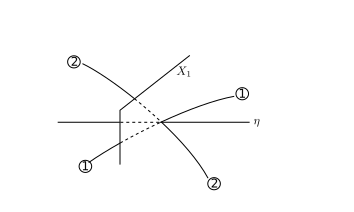
\includegraphics{figure/fig76-3.1_1.eps}
\caption{Local zero set of $\hat{g}$ ($\hat{k}$ odd).}
\end{figure}


As $\hat{k}$ is odd and the mapping $n \to \eta^{\hat{k}}$ is a
homeomorphism of $\mathbb{R}$, the corresponding curve $(\mu(t),
x(t))$ with $\mu(t) = \eta^{\hat{k}}(t)$ in the local zero set of
$\hat{f}$ is also located on both sides of the hyperplane $\{0\}
\times X_{1}$ in $\mathbb{R} \times X_{1}$. Of course,
$$
\frac{d}{dt} (\mu(t), x(t)) |_{t=0} = (0, \frac{dx}{dt} (0)).
$$

But $\frac{dx}{dt}(0) \neq 0$, because the non-zero vector,
$\left(\frac{d\eta}{dt}(0), \frac{dx}{dt} (0)\right)$ is in the zero
set of the mapping (\ref{chap3-eq3.25}), which does not contain the
line $(\eta, 0)$\footnote{See Proposition \ref{chap3-prop3.1} later}
As a result, each curve $(\mu(t), x(t))$ in the local zero set of
$\hat{f}$ is tangent to the hyperplane $\{0\} \times X_{1}$ at the
origin. Replacing the hyperplane $\{0\} \times X_{1}$ in $\mathbb{R}
\times X_{1}$ by the hyperplane $\{0\} \times X$ in $\mathbb{R} \times
X$, these\pageoriginale statements remain readily valid as concerns
the local zero set of the mapping $G$.
\begin{figure}[H]
\centering
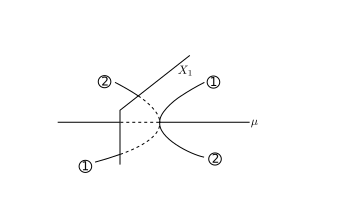
\includegraphics{figure/fig76-3.2_1.eps}
\caption{Local zero set of $\hat{f}$ ($\hat{k}$ odd).}
\end{figure}


Assume next that $\hat{k}$ is {\em even} and the both mappings
(\ref{chap3-eq3.26}) verify the condition $(\mathbb{R}-N.D.)$. As
before, if $t \to (\eta(t), x(t))$ is one of the curves in the local
zero set of $\hat{g}_{1}$ or $\hat{g}_{-1}$, one has 
$$
\frac{d\eta}{dt}(0) \neq 0, \frac{dx}{dt} (0) \neq 0.
$$

In particular, the corresponding curve $(\mu(t), x(t))$ with $\mu(t) =
\sigma \eta^{\hat{k}}(t)$ in the local zero set of $\hat{f}$ is
tangent to the hyperplane $\{0\} \times X_{1}$ at the origin. But, as
$\sigma \eta^{\hat{k}}(t)$ does {\em not} change sign for $t$ varying
around 0, this curve is {\em located on one side} of the hyperplane
$\{0\} \times X_{1}$ in $\mathbb{R} \times X_{1}$. Again, replacing
the hyperplane $\{0\} \times X_{1}$ in $\mathbb{R} \times X_{1}$ by
the hyperplane $\{0\} \times X$ in $\mathbb{R} \times X$, these
statements\pageoriginale remain readily valid as concerns the local
zero set of the mapping $G$.
\begin{figure}[H]
\centering
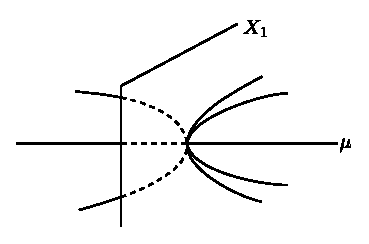
\includegraphics{figure/fig76-3.3_1.eps}
\caption{Local zero set of $\hat{f}$ ($\hat{k}$ even)}
\end{figure}

We are now going to relate the assumptions we make for solving the
problem after changing the parameter $\mu$ into $\eta^{\hat{k}}$ or
$\sigma \eta^{\hat{k}}$ to the assumptions we made earlier to solve it
without changing $\mu$. First, observe that the integer $\hat{k}$
characterized by (\ref{chap3-eq3.18}). Indeed, $\hat{k}$ is
independent of the choice of the space $\hat{Y}_{1}$ and from the
definitions, it is immediate that $\hat{Y}_{1}$ can be chosen so that 
\begin{equation*}
\hat{Y}_{1} \supset Y_{1}\tag{3.28}\label{chap3-eq3.28}
\end{equation*}
where $Y_{1}$ is any space chosen for defining $k$. By the same
arguments, note\pageoriginale that
\begin{equation*}
\hat{k}_{1} \leq k_{1}, \hat{k}^{1} \leq k^{1},\tag{3.29}\label{chap3-eq3.29}
\end{equation*}
(cf. (\ref{chap3-eq3.9})-(\ref{chap3-eq3.10}) and
(\ref{chap3-eq3.22})-(\ref{chap3-eq3.23})). But we shall see that the
integers $k$ and $\hat{k}$ {\em must coincide} for the mappings
(\ref{chap3-eq3.25}) or \ref{chap3-eq3.27} to verify the condition
$(\mathbb{R}-N.D.)$ when $n \geq 1$. This is proved in
\begin{proposition}\label{chap3-prop3.1}
Assume $\hat{k}$ is odd (resp. even). Then, the mapping
(\ref{chap3-eq3.25}) (resp. $(3.27)_{1}$ and $(3.27)_{-1}$) erifies
the condition $(\mathbb{R}-N.D.)$ is and only if
\begin{equation*}
\hat{Q}_{1}D_{x}^{\hat{k}}F(0) \cdot (x)^{\hat{k}} \neq 0,\tag{3.30}\label{chap3-eq3.30}
\end{equation*}
for every $x \epsilon X_{1} - \{0\}$ and the mapping
\begin{equation*}
x \epsilon X_{1} \to Q_{1}D_{x}^{\hat{k}}F(0) \cdot (x)^{\hat{k}}
\epsilon Y_{1},\tag{3.31}\label{chap3-eq3.31}
\end{equation*}
verifies the condition $(\mathbb{R}-N.D.)$. In particular, when $n
\geq 1$, one must have $\hat{k} = k$. When $n = 0$, the condition
(\ref{chap3-eq3.30}) holds by the definition of $\hat{k}, k$ is not
defined and $Y_{1} = \{0\}$ so that the mapping (\ref{chap3-eq3.31})
verifies the condition $(\mathbb{R}-N.D.)$ trivially.
\end{proposition}

\begin{proof}
We prove the equivalence when $\hat{k}$ is odd. When $\hat{k}$ is
even, the proof is identical and left to the reader.

The condition (\ref{chap3-eq3.30}) is necessary. Indeed, if
$\hat{Q}_{1}D_{x}^{\hat{k}}F(0) \cdot (x)^{\hat{k}} = 0$ for some $x
\epsilon X_{1} - \{0\}$, the line $\{0\} \times \mathbb{R}x$ is in the
zero set of the mapping (\ref{chap3-eq3.25}) whose derivaitve at $(0,
x) \epsilon \mathbb{R} \times X_{1}$ is
$$
(\eta' , x') \epsilon \mathbb{R} \times X_{1} \to
\hat{k}\hat{Q}_{1}D_{x}^{\hat{k}}F(0) \cdot ((x)^{\hat{k}-1}, x')
\epsilon \hat{Y}_{1}.
$$

Its\pageoriginale null-space contains the two-dimensional subspace
$\mathbb{R} (1, 0) \oplus (\{0\} \times \mathbb{R}x)$ and hence its
range is of dimension $\leq \hat{n} - 1$ so that the condition
$(\mathbb{R}-N.D.)$ fails.

Now, we prove that the mapping (\ref{chap3-eq3.31}) verifies the
condition $(\mathbb{R}-N.D.)$. As our assumptions are independent of
the space $\hat{Y}_{1}$, we can suppose that
\begin{equation*}
\hat{Y}_{1} = \mathbb{R} y^{0} \oplus Y_{1}.\tag{3.32}\label{chap3-eq3.32}
\end{equation*}

If so, $\hat{Q}_{1} y^{0} = y^{0}, Q_{1}\hat{Q}_{1} = Q_{1}$ and the
operator $\hat{Q}_{1} - Q_{1}$ is the projection onto the space
$\mathbb{R} y^{0}$ associated with the decomposition $Y = \mathbb{R}
y^{0} \oplus (Y_{1} \oplus Range D_{x}F(0))$. Then, the mapping
(\ref{chap3-eq3.25}) becomes 
$$
(\eta, x) \epsilon \mathbb{R} \times X_{1} \to \hat{k}! \eta^{\hat{k}}
y^{0} + \hat{Q}_{1}D_{x}^{\hat{k}}F(0) \cdot (x)^{\hat{k}} \epsilon \hat{Y}_{1}.
$$

Let now $x$ be a non-zero element of the zero set of the mapping
(\ref{chap3-eq3.31}) so that $\hat{Q}_{1}D_{x}^{\hat{k}}F(0) \cdot
(x)^{\hat{k}} = (\hat{Q}_{1} - Q_{1}) D_{x}^{\hat{k}}F(0) \cdot
(x)^{\hat{k}}$, and, from the above, the right hand side is collinear
with $y^{0}$. Therefore
$$
\hat{Q}_{1}D_{x}^{\hat{k}}F(0) \cdot (x)^{\hat{k}} = \lambda y^{0},
$$
for some real number $\lambda$. As $\hat{k}$ is odd, there is $\eta
\epsilon \mathbb{R}$ such that $\hat{k}! \eta^{\hat{k}} = -\lambda$
and the pair $(\eta, x) \epsilon \mathbb{R} \times X_{1}$ is in the
zero set of the mapping (\ref{chap3-eq3.25}). Let $y \epsilon Y_{1}$
be given. In particular, $y \epsilon \hat{Y}_{1}$
(cf. \ref{chap3-eq3.32}) and there is a pair $(\eta', x') \epsilon
\mathbb{R} \times X_{1}$ such that
$$
\hat{k} (\hat{k}!) \eta^{\hat{k} - 1} \eta' y^{0} + 
\hat{k}\hat{Q}_{1}D_{x}^{\hat{k}}F(0) \cdot ((x)^{\hat{k} - 1}, x') = y.
$$

Taking the projection onto $Y_{1}$, we find
$$
\hat{k}Q_{1} D_{x}^{\hat{k}}F(0) \bullet ((x)^{\hat{k}-1}, x') = y,
$$\pageoriginale
which proves our assertion.

Conversely, let $(\eta, x) \epsilon \mathbb{R} \times X_{1}$ be a
non-zero element of the zero set of the mapping
(\ref{chap3-eq3.25}). Observe that $\eta \neq 0$ from
(\ref{chap3-eq3.30}) and it is obvious that $x \neq 0$. Taking the
projection onto $Y_{1}$, we find that $x$ is in the zero set of the
mapping (\ref{chap3-eq3.31}). Let $\hat{y} \epsilon \hat{Y}_{1}$ be
given and set $y = Q_{1}\hat{y}$. By hypothesis, there exists $x'
\epsilon X_{1}$ such that $\hat{k}Q_{1} D_{x}^{\hat{k}}F(0) \cdot
((x)^{\hat{k}-1}, x') = y$. As $(\hat{Q}_{1} - Q_{1})$ is the
projection onto the space $\mathbb{R}y^{0}$ and by definition of $y$, we
find
$$
\hat{k} \hat{Q}_{1} D_{x}^{\hat{k}}F(0) \cdot ((x)^{\hat{k} - 1}, x')
= \hat{y} + \lambda y^{0},
$$
for some real number $\lambda$. Setting
$$
\eta' = -\lambda / \hat{k} (\hat{k}!) \eta^{\hat{k}-1},
$$
it is clear that
$$
\hat{k}(\hat{k}!)^{\hat{k}-1} \eta'y^{0} + \hat{k}\hat{Q}_{1}
D_{x}^{\hat{k}}F(0) \cdot ((x)^{\hat{k}-1}, x') = \hat{y},
$$
so that the mapping (\ref{chap3-eq3.25}) verifies the condition
$(\mathbb{R}-N.D.).$

The end of our assertion is obvious. If $n \geq 1$, we already know
that $\hat{k} \leq k$ and, if $\hat{k} < k$, one has
$$
Q_{1} D_{x}^{\hat{k}}F(0) |_{(X_{1})^{\hat{k}}} = 0,
$$
by definition of $k$, which contradicts the fact that the mapping
(\ref{chap3-eq3.31}) verifies the condition $(\mathbb{R}-N.D.)$. When
$n = 0$, the space $\hat{Y}_{1}$ is one-dimensional (i.e. $\hat{n} =
1$) and the condition (\ref{chap3-eq3.30}) is then automatically
satisfied\pageoriginale by definition of $\hat{k}$.
\end{proof}

To sum up, the local zero set of the mapping $G$ (\ref{chap3-eq3.3}) can
be found after changing the parameter $\mu$ into $\eta^{\hat{k}}$
under the conditions 
\begin{enumerate}
\item[a)] $D_{x}F(0)$ is a Fredholm operator with index 0,

\item[b)] $\hat{k} \leq \hat{k}_{1} + \hat{k}^{1} - 2$,

\item[c)] $\hat{Q}_{1} D_{x}^{\hat{k}}F(0) \cdot (x)^{\hat{k}} \neq 0$
  for every $x \epsilon X_{1} - \{0\}$,

\item[d)] the mapping
$$
x \epsilon X_{1} \to Q_{1}D_{x}^{\hat{k}}F(0) \cdot (x)^{\hat{k}}
\epsilon Y_{1},
$$
verifies the condition $(\mathbb{R}-N.D.)$.
\end{enumerate}

In any case, these assumptions are {\em stronger} than those made when
the local zero set of $G$ is determined without chaging the parameter
$\mu$ (see in particular (\ref{chap3-eq3.29}) and recall that
$\hat{k}$ must equal $k$ when $n \geq 1$) and the conclusions are {\em
  not as precise}: The number of curves is found to be $\leq
\hat{k}^{\hat{n}} = \hat{k}^{n+1}$. When $n \geq 1$, this upper bound
is nothing but $k^{n+1}$ (but we know that it is actually $k^{n}$) and
$\hat{k}$ when $n = 0$ (but we know that there is exactly one
curve). The regularity we obtain is of class $C^{m-\hat{k}+1}$ at the
origin and of class $C^{m}$ away from it, which agress with the
previous result if $n \geq 1$ (since $\hat{k} = k$) but is not as good
when $n = 0$ (the curve is actually of class $C^{m}$ at the
origin). However, the additional information which may be of interest
is the {\em location} of {\em the curves} in the space $\mathbb{R}
\times X$. In particular, when $n = 0$,\pageoriginale the reader can
immediately deduce, from the appropriate discussion given before, that
the origin is a {\em ``turning point''} when $\hat{k}$ is {\em even}
and a {\em ``hysteresis point''} when $\hat{k}$ is {\em odd}. When $n
\geq 1$, bifurcation may occur but the origin can be an isolated
solutoion as well (see the example given in Remark \ref{chap3-rem3.1}).
